\documentclass[twoside]{book}

% Packages required by doxygen
\usepackage{fixltx2e}
\usepackage{calc}
\usepackage{doxygen}
\usepackage{graphicx}
\usepackage[utf8]{inputenc}
\usepackage{makeidx}
\usepackage{multicol}
\usepackage{multirow}
\PassOptionsToPackage{warn}{textcomp}
\usepackage{textcomp}
\usepackage[nointegrals]{wasysym}
\usepackage[table]{xcolor}

% Font selection
\usepackage[T1]{fontenc}
\usepackage{mathptmx}
\usepackage[scaled=.90]{helvet}
\usepackage{courier}
\usepackage{amssymb}
\usepackage{sectsty}
\renewcommand{\familydefault}{\sfdefault}
\allsectionsfont{%
  \fontseries{bc}\selectfont%
  \color{darkgray}%
}
\renewcommand{\DoxyLabelFont}{%
  \fontseries{bc}\selectfont%
  \color{darkgray}%
}
\newcommand{\+}{\discretionary{\mbox{\scriptsize$\hookleftarrow$}}{}{}}

% Page & text layout
\usepackage{geometry}
\geometry{%
  a4paper,%
  top=2.5cm,%
  bottom=2.5cm,%
  left=2.5cm,%
  right=2.5cm%
}
\tolerance=750
\hfuzz=15pt
\hbadness=750
\setlength{\emergencystretch}{15pt}
\setlength{\parindent}{0cm}
\setlength{\parskip}{0.2cm}
\makeatletter
\renewcommand{\paragraph}{%
  \@startsection{paragraph}{4}{0ex}{-1.0ex}{1.0ex}{%
    \normalfont\normalsize\bfseries\SS@parafont%
  }%
}
\renewcommand{\subparagraph}{%
  \@startsection{subparagraph}{5}{0ex}{-1.0ex}{1.0ex}{%
    \normalfont\normalsize\bfseries\SS@subparafont%
  }%
}
\makeatother

% Headers & footers
\usepackage{fancyhdr}
\pagestyle{fancyplain}
\fancyhead[LE]{\fancyplain{}{\bfseries\thepage}}
\fancyhead[CE]{\fancyplain{}{}}
\fancyhead[RE]{\fancyplain{}{\bfseries\leftmark}}
\fancyhead[LO]{\fancyplain{}{\bfseries\rightmark}}
\fancyhead[CO]{\fancyplain{}{}}
\fancyhead[RO]{\fancyplain{}{\bfseries\thepage}}
\fancyfoot[LE]{\fancyplain{}{}}
\fancyfoot[CE]{\fancyplain{}{}}
\fancyfoot[RE]{\fancyplain{}{\bfseries\scriptsize Generated on Mon Dec 28 2015 16\+:07\+:58 for Fisherman Locator by Doxygen }}
\fancyfoot[LO]{\fancyplain{}{\bfseries\scriptsize Generated on Mon Dec 28 2015 16\+:07\+:58 for Fisherman Locator by Doxygen }}
\fancyfoot[CO]{\fancyplain{}{}}
\fancyfoot[RO]{\fancyplain{}{}}
\renewcommand{\footrulewidth}{0.4pt}
\renewcommand{\chaptermark}[1]{%
  \markboth{#1}{}%
}
\renewcommand{\sectionmark}[1]{%
  \markright{\thesection\ #1}%
}

% Indices & bibliography
\usepackage{natbib}
\usepackage[titles]{tocloft}
\setcounter{tocdepth}{3}
\setcounter{secnumdepth}{5}
\makeindex

% Hyperlinks (required, but should be loaded last)
\usepackage{ifpdf}
\ifpdf
  \usepackage[pdftex,pagebackref=true]{hyperref}
\else
  \usepackage[ps2pdf,pagebackref=true]{hyperref}
\fi
\hypersetup{%
  colorlinks=true,%
  linkcolor=blue,%
  citecolor=blue,%
  unicode%
}

% Custom commands
\newcommand{\clearemptydoublepage}{%
  \newpage{\pagestyle{empty}\cleardoublepage}%
}


%===== C O N T E N T S =====

\begin{document}

% Titlepage & ToC
\hypersetup{pageanchor=false,
             bookmarks=true,
             bookmarksnumbered=true,
             pdfencoding=unicode
            }
\pagenumbering{roman}
\begin{titlepage}
\vspace*{7cm}
\begin{center}%
{\Large Fisherman Locator \\[1ex]\large 0.\+9 }\\
\vspace*{1cm}
{\large Generated by Doxygen 1.8.7}\\
\vspace*{0.5cm}
{\small Mon Dec 28 2015 16:07:58}\\
\end{center}
\end{titlepage}
\clearemptydoublepage
\tableofcontents
\clearemptydoublepage
\pagenumbering{arabic}
\hypersetup{pageanchor=true}

%--- Begin generated contents ---
\chapter{Main Page}
\label{index}\hypertarget{index}{}{\itshape Find your lozenges around the globe.}

This website helps you fo find the famous Fisherman's Friends (R) Lozenges.

\subsubsection*{Aim of the project}

The final Aim of the project is to develop a website that allows its users to get informed about which shops sell the Fisherman's Friends (R) Lozenges, which are the best equipped and allow them to rate the shops and add new ones. While this is the final aim, in this scope the requisites where far less ambitious, so the website presents some bare minimum functionalities and should be considered as a proof of concept.

\subsubsection*{Structure of the website}

The website implements a classic M\+V\+C pattern, as asked in the requirements. The structure can be seen in the doxygen documentation attached in the project itself.

\subsubsection*{Current level of functionality}

In the current state (version 0.\+9) the website has the following capabilities\+:


\begin{DoxyItemize}
\item Signup system\+: a user can sign up;
\item Login system\+: a registered user can log in;
\item Shops reporting\+: a logged user can add a new shop to the database;
\item Shops research\+: a user can search shops (match by shop name or city);
\item Profile view\+: a logged user can see its profile informatons;
\item Shops removal\+: an admin can remove shops.
\end{DoxyItemize}

\subsubsection*{Project requirements}

\begin{TabularC}{2}
\hline
\rowcolor{lightgray}{\bf Requirement }&\PBS\centering {\bf Details  }\\\cline{1-2}
H\+T\+M\+L &\PBS\centering {\itshape Y\+E\+S} \\\cline{1-2}
C\+S\+S &\PBS\centering {\itshape Y\+E\+S} \\\cline{1-2}
P\+H\+P &\PBS\centering {\itshape Y\+E\+S} \\\cline{1-2}
My\+S\+Q\+L &\PBS\centering {\itshape Y\+E\+S} \\\cline{1-2}
two roles at least &\PBS\centering {\itshape Yes\+: admin, registered user and not registered user} \\\cline{1-2}
transactions &\PBS\centering {\itshape Yes, \hyperlink{classShopModel_ae035aa872e97c08247d203f90e228fe2}{Shop\+Model\+::remove\+Shop()}} \\\cline{1-2}
Ajax &\PBS\centering {\itshape Yes\+: \hyperlink{classBasePageController_a96ace79928e80d29e6560b1fb965e859}{Base\+Page\+Controller\+::load\+Page\+Ajax\+Search\+Shop()}, \hyperlink{classPresenter_a02088a50a3134097a1b785b0315937b6}{Presenter\+::json()}} \\\cline{1-2}
Log in credentials &\PBS\centering {\itshape Admin -\/$>$ username\+: admin, password\+: admin} \\\cline{1-2}
\end{TabularC}

\chapter{Hierarchical Index}
\section{Class Hierarchy}
This inheritance list is sorted roughly, but not completely, alphabetically\+:\begin{DoxyCompactList}
\item \contentsline{section}{Controller}{\pageref{classController}}{}
\begin{DoxyCompactList}
\item \contentsline{section}{Base\+Page\+Controller}{\pageref{classBasePageController}}{}
\end{DoxyCompactList}
\item \contentsline{section}{Footer}{\pageref{classFooter}}{}
\item \contentsline{section}{Head}{\pageref{classHead}}{}
\item \contentsline{section}{Header}{\pageref{classHeader}}{}
\item \contentsline{section}{Link}{\pageref{classLink}}{}
\item \contentsline{section}{Login\+Form}{\pageref{classLoginForm}}{}
\item \contentsline{section}{Model}{\pageref{classModel}}{}
\begin{DoxyCompactList}
\item \contentsline{section}{D\+B\+Model}{\pageref{classDBModel}}{}
\begin{DoxyCompactList}
\item \contentsline{section}{Login\+Model}{\pageref{classLoginModel}}{}
\item \contentsline{section}{Sign\+Up\+Model}{\pageref{classSignUpModel}}{}
\end{DoxyCompactList}
\item \contentsline{section}{Error\+Model}{\pageref{classErrorModel}}{}
\item \contentsline{section}{Home\+Model}{\pageref{classHomeModel}}{}
\end{DoxyCompactList}
\item \contentsline{section}{Nav}{\pageref{classNav}}{}
\item \contentsline{section}{Presenter}{\pageref{classPresenter}}{}
\item \contentsline{section}{Sign\+Up\+Form}{\pageref{classSignUpForm}}{}
\item \contentsline{section}{User}{\pageref{classUser}}{}
\end{DoxyCompactList}

\chapter{Class Index}
\section{Class List}
Here are the classes, structs, unions and interfaces with brief descriptions\+:\begin{DoxyCompactList}
\item\contentsline{section}{\hyperlink{classBasePageController}{Base\+Page\+Controller} }{\pageref{classBasePageController}}{}
\item\contentsline{section}{\hyperlink{classController}{Controller} }{\pageref{classController}}{}
\item\contentsline{section}{\hyperlink{classDBModel}{D\+B\+Model} }{\pageref{classDBModel}}{}
\item\contentsline{section}{\hyperlink{classErrorModel}{Error\+Model} }{\pageref{classErrorModel}}{}
\item\contentsline{section}{\hyperlink{classFooter}{Footer} }{\pageref{classFooter}}{}
\item\contentsline{section}{\hyperlink{classForm}{Form} }{\pageref{classForm}}{}
\item\contentsline{section}{\hyperlink{classGenericModel}{Generic\+Model} }{\pageref{classGenericModel}}{}
\item\contentsline{section}{\hyperlink{classGenericView}{Generic\+View} }{\pageref{classGenericView}}{}
\item\contentsline{section}{\hyperlink{classHead}{Head} }{\pageref{classHead}}{}
\item\contentsline{section}{\hyperlink{classHeader}{Header} }{\pageref{classHeader}}{}
\item\contentsline{section}{\hyperlink{classHomeModel}{Home\+Model} }{\pageref{classHomeModel}}{}
\item\contentsline{section}{\hyperlink{classLink}{Link} }{\pageref{classLink}}{}
\item\contentsline{section}{\hyperlink{classModel}{Model} }{\pageref{classModel}}{}
\item\contentsline{section}{\hyperlink{classNav}{Nav} }{\pageref{classNav}}{}
\item\contentsline{section}{\hyperlink{classPresenter}{Presenter} }{\pageref{classPresenter}}{}
\item\contentsline{section}{\hyperlink{classShopModel}{Shop\+Model} }{\pageref{classShopModel}}{}
\item\contentsline{section}{\hyperlink{classUser}{User} }{\pageref{classUser}}{}
\item\contentsline{section}{\hyperlink{classUserAccessModel}{User\+Access\+Model} }{\pageref{classUserAccessModel}}{}
\end{DoxyCompactList}

\chapter{Class Documentation}
\hypertarget{classBasePageController}{\section{Base\+Page\+Controller Class Reference}
\label{classBasePageController}\index{Base\+Page\+Controller@{Base\+Page\+Controller}}
}


Inheritance diagram for Base\+Page\+Controller\+:\nopagebreak
\begin{figure}[H]
\begin{center}
\leavevmode
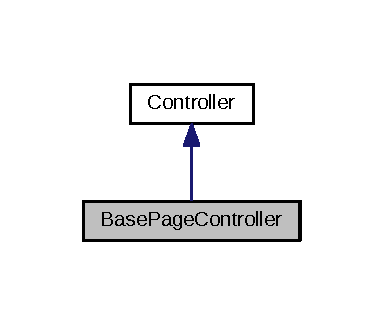
\includegraphics[width=184pt]{classBasePageController__inherit__graph}
\end{center}
\end{figure}


Collaboration diagram for Base\+Page\+Controller\+:\nopagebreak
\begin{figure}[H]
\begin{center}
\leavevmode
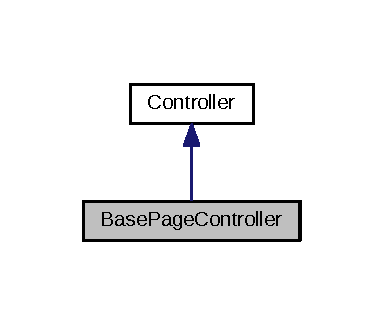
\includegraphics[width=184pt]{classBasePageController__coll__graph}
\end{center}
\end{figure}
\subsection*{Public Member Functions}
\begin{DoxyCompactItemize}
\item 
\hypertarget{classBasePageController_a483998015a3518d49897d271de2e3c2d}{{\bfseries \+\_\+\+\_\+construct} (\&\$request)}\label{classBasePageController_a483998015a3518d49897d271de2e3c2d}

\item 
\hyperlink{classBasePageController_a66084d1db3fcc8a5cb1f44cd82b7948a}{load\+Page\+Home} ()
\item 
\hyperlink{classBasePageController_aae6760084899d261e8f19f8dc2cbfd30}{load\+Page\+Signup} ()
\item 
\hyperlink{classBasePageController_a36cdd7c6a038c2664b333fbf8de6383a}{load\+Page\+Login} ()
\item 
\hyperlink{classBasePageController_ae7d620e0d251d06407cfe960cafe3d57}{load\+Page\+Logout} ()
\item 
\hyperlink{classBasePageController_aecf3ccde53aaa9b780feb5e12f2904ea}{load\+Page\+Addshop} ()
\item 
\hyperlink{classBasePageController_ae7ecc6f491f580059698d1a1a8e8d9ac}{load\+Page\+Help} ()
\item 
\hyperlink{classBasePageController_affa5617be55ed9bf233fd7bd1b2e19c9}{load\+Page\+Profile} ()
\item 
\hyperlink{classBasePageController_ad63921678e571dbd0a37d3afd6b55f5a}{load\+Page\+Remove\+Shop} ()
\item 
\hyperlink{classBasePageController_a96ace79928e80d29e6560b1fb965e859}{load\+Page\+Ajax\+Search\+Shop} ()
\item 
\hyperlink{classBasePageController_a07d3e03b8e2ec5cc698f057a3496c14b}{load\+Page\+Err404} ()
\item 
\hyperlink{classBasePageController_a9ecd03fb676ab32ee9c2cb4e412757cc}{load\+Page\+Err403} ()
\item 
\hyperlink{classBasePageController_a877c4f32b7d39e566f7832aef94c2f11}{set\+Signup\+Fields} ()
\item 
\hyperlink{classBasePageController_a777f34065716ce7f7706ea745fbdd254}{set\+Warning} (\$field)
\item 
\hyperlink{classBasePageController_a56e85dfb915144831cf39435b88774f5}{check\+Fields\+Sign\+Up} (\hyperlink{classUserAccessModel}{User\+Access\+Model} \$model)
\item 
\hyperlink{classBasePageController_a2aaad6f0fa836c9d7e6d9df5974cb4a7}{get\+Date} (\$year=\char`\"{}\char`\"{}, \$month=\char`\"{}\char`\"{}, \$day=\char`\"{}\char`\"{})
\item 
\hyperlink{classBasePageController_ade6dad738c6fce22cf8b44028628090d}{check\+Char\+Digit} (\$field, \$value, \$length=-\/1)
\item 
\hyperlink{classBasePageController_ab4d71880bb1227a04df998de6cfc0f34}{check\+Char\+Spaces} (\$field, \$value, \$length=-\/1)
\item 
\hyperlink{classBasePageController_aaf4afedf5bb714c46c29e007eb095e55}{check\+Composed\+Strings} (\$field, \$value, \$symbols=\char`\"{}a-\/z\+A-\/Z0-\/9 ',.-\/°\char`\"{}, \$length=-\/1)
\item 
\hyperlink{classBasePageController_ad79d970cb91298dfa2206bfe22516618}{check\+Decimal} (\$field, \$value)
\item 
\hyperlink{classBasePageController_a6829b94ed721619b43879475c75b8fc8}{check\+Password} (\$field, \$value)
\item 
\hyperlink{classBasePageController_a5a0788181caf223a4ce208702c93e0c8}{check\+Email} (\$field, \$value)
\item 
\hyperlink{classBasePageController_a6f1a0a900ee8f95b6b6f12c52272a9a7}{check\+Date} (\$field, \$value)
\item 
\hyperlink{classBasePageController_ac0083ad81bbac88f3ca4bdf258566a07}{concat\+Error\+Array} (\$error)
\item 
\hyperlink{classBasePageController_a153a1dcf2e23be9499f8083828671c26}{set\+Addshop\+Data} ()
\item 
\hyperlink{classBasePageController_aa71c4d8a5aa7b90d2074e511fe4ddcc2}{check\+Fields\+Addshop} (\$data)
\end{DoxyCompactItemize}
\subsection*{Public Attributes}
\begin{DoxyCompactItemize}
\item 
\hypertarget{classBasePageController_a35247fc10b6367518b2232ea4d5ca90a}{const {\bfseries P\+A\+S\+S\+W\+O\+R\+D\+\_\+\+M\+I\+N\+\_\+\+L\+E\+N} = 6}\label{classBasePageController_a35247fc10b6367518b2232ea4d5ca90a}

\item 
\hypertarget{classBasePageController_acc0b220a790dddcd88a8ff7fd8fb88c9}{const {\bfseries U\+S\+E\+R\+\_\+\+M\+I\+N\+\_\+\+L\+E\+N} = 5}\label{classBasePageController_acc0b220a790dddcd88a8ff7fd8fb88c9}

\item 
\hypertarget{classBasePageController_a038012b54b56da5c27dbfc773ce75b00}{const {\bfseries F\+I\+E\+L\+D\+\_\+\+M\+I\+N\+\_\+\+L\+E\+N} = 1}\label{classBasePageController_a038012b54b56da5c27dbfc773ce75b00}

\end{DoxyCompactItemize}
\subsection*{Additional Inherited Members}


\subsection{Detailed Description}
Handles the pages, the checks, sanitizes the input and more.

\begin{DoxyAuthor}{Author}
Fabio Colella. 
\end{DoxyAuthor}


\subsection{Member Function Documentation}
\hypertarget{classBasePageController_ade6dad738c6fce22cf8b44028628090d}{\index{Base\+Page\+Controller@{Base\+Page\+Controller}!check\+Char\+Digit@{check\+Char\+Digit}}
\index{check\+Char\+Digit@{check\+Char\+Digit}!Base\+Page\+Controller@{Base\+Page\+Controller}}
\subsubsection[{check\+Char\+Digit}]{\setlength{\rightskip}{0pt plus 5cm}Base\+Page\+Controller\+::check\+Char\+Digit (
\begin{DoxyParamCaption}
\item[{}]{\$field, }
\item[{}]{\$value, }
\item[{}]{\$length = {\ttfamily -\/1}}
\end{DoxyParamCaption}
)}}\label{classBasePageController_ade6dad738c6fce22cf8b44028628090d}
Helper function to check if strings contain only chars and digits.


\begin{DoxyParams}[1]{Parameters}
string & {\em \$field} & the name of the field. \\
\hline
string & {\em \$value} & the value of the field. \\
\hline
int & {\em \$length} & (optional) checks also the lenghts of the value. \\
\hline
\end{DoxyParams}
\begin{DoxyReturn}{Returns}
boolean true if the test is passed. 
\end{DoxyReturn}
\hypertarget{classBasePageController_ab4d71880bb1227a04df998de6cfc0f34}{\index{Base\+Page\+Controller@{Base\+Page\+Controller}!check\+Char\+Spaces@{check\+Char\+Spaces}}
\index{check\+Char\+Spaces@{check\+Char\+Spaces}!Base\+Page\+Controller@{Base\+Page\+Controller}}
\subsubsection[{check\+Char\+Spaces}]{\setlength{\rightskip}{0pt plus 5cm}Base\+Page\+Controller\+::check\+Char\+Spaces (
\begin{DoxyParamCaption}
\item[{}]{\$field, }
\item[{}]{\$value, }
\item[{}]{\$length = {\ttfamily -\/1}}
\end{DoxyParamCaption}
)}}\label{classBasePageController_ab4d71880bb1227a04df998de6cfc0f34}
Helper function to check if strings contain only chars and spaces. 
\begin{DoxyParams}[1]{Parameters}
string & {\em \$field} & the name of the field. \\
\hline
string & {\em \$value} & the value of the field. \\
\hline
int & {\em \$length} & (optional) checks also the lenghts of the value. \\
\hline
\end{DoxyParams}
\begin{DoxyReturn}{Returns}
boolean true if the test is passed. 
\end{DoxyReturn}
\hypertarget{classBasePageController_aaf4afedf5bb714c46c29e007eb095e55}{\index{Base\+Page\+Controller@{Base\+Page\+Controller}!check\+Composed\+Strings@{check\+Composed\+Strings}}
\index{check\+Composed\+Strings@{check\+Composed\+Strings}!Base\+Page\+Controller@{Base\+Page\+Controller}}
\subsubsection[{check\+Composed\+Strings}]{\setlength{\rightskip}{0pt plus 5cm}Base\+Page\+Controller\+::check\+Composed\+Strings (
\begin{DoxyParamCaption}
\item[{}]{\$field, }
\item[{}]{\$value, }
\item[{}]{\$symbols = {\ttfamily \char`\"{}a-\/zA-\/Z0-\/9~',.-\/°\char`\"{}}, }
\item[{}]{\$length = {\ttfamily -\/1}}
\end{DoxyParamCaption}
)}}\label{classBasePageController_aaf4afedf5bb714c46c29e007eb095e55}
Helper function to check if strings contain only certain symbols.


\begin{DoxyParams}[1]{Parameters}
string & {\em \$field} & the name of the field. \\
\hline
string & {\em \$value} & the value of the field. \\
\hline
string & {\em \$symbols} & A list of symbols allowed, default\+: \char`\"{}a-\/z\+A-\/\+Z0-\/9 ',.-\/°\char`\"{}. \\
\hline
int & {\em \$length} & (optional) checks also the lenghts of the value. \\
\hline
\end{DoxyParams}
\begin{DoxyReturn}{Returns}
boolean true if the test is passed. 
\end{DoxyReturn}
\hypertarget{classBasePageController_a6f1a0a900ee8f95b6b6f12c52272a9a7}{\index{Base\+Page\+Controller@{Base\+Page\+Controller}!check\+Date@{check\+Date}}
\index{check\+Date@{check\+Date}!Base\+Page\+Controller@{Base\+Page\+Controller}}
\subsubsection[{check\+Date}]{\setlength{\rightskip}{0pt plus 5cm}Base\+Page\+Controller\+::check\+Date (
\begin{DoxyParamCaption}
\item[{}]{\$field, }
\item[{}]{\$value}
\end{DoxyParamCaption}
)}}\label{classBasePageController_a6f1a0a900ee8f95b6b6f12c52272a9a7}
Checks that the date is in an appropriate format (Y\+Y\+Y\+Y-\/\+M\+M-\/\+D\+D).


\begin{DoxyParams}[1]{Parameters}
string & {\em \$field} & the name of the field. \\
\hline
string & {\em \$value} & the value of the field. \\
\hline
\end{DoxyParams}
\begin{DoxyReturn}{Returns}
boolean true if the test is passed. 
\end{DoxyReturn}
\hypertarget{classBasePageController_ad79d970cb91298dfa2206bfe22516618}{\index{Base\+Page\+Controller@{Base\+Page\+Controller}!check\+Decimal@{check\+Decimal}}
\index{check\+Decimal@{check\+Decimal}!Base\+Page\+Controller@{Base\+Page\+Controller}}
\subsubsection[{check\+Decimal}]{\setlength{\rightskip}{0pt plus 5cm}Base\+Page\+Controller\+::check\+Decimal (
\begin{DoxyParamCaption}
\item[{}]{\$field, }
\item[{}]{\$value}
\end{DoxyParamCaption}
)}}\label{classBasePageController_ad79d970cb91298dfa2206bfe22516618}
Helper function to check if strings contain only decimal numbers.


\begin{DoxyParams}[1]{Parameters}
string & {\em \$field} & the name of the field. \\
\hline
string & {\em \$value} & the value of the field. \\
\hline
\end{DoxyParams}
\begin{DoxyReturn}{Returns}
boolean true if the test is passed. 
\end{DoxyReturn}
\hypertarget{classBasePageController_a5a0788181caf223a4ce208702c93e0c8}{\index{Base\+Page\+Controller@{Base\+Page\+Controller}!check\+Email@{check\+Email}}
\index{check\+Email@{check\+Email}!Base\+Page\+Controller@{Base\+Page\+Controller}}
\subsubsection[{check\+Email}]{\setlength{\rightskip}{0pt plus 5cm}Base\+Page\+Controller\+::check\+Email (
\begin{DoxyParamCaption}
\item[{}]{\$field, }
\item[{}]{\$value}
\end{DoxyParamCaption}
)}}\label{classBasePageController_a5a0788181caf223a4ce208702c93e0c8}
Helper function to check if the string is a valid email address.


\begin{DoxyParams}[1]{Parameters}
string & {\em \$field} & the name of the field. \\
\hline
string & {\em \$value} & the value of the field. \\
\hline
\end{DoxyParams}
\begin{DoxyReturn}{Returns}
boolean true if the test is passed. 
\end{DoxyReturn}
\hypertarget{classBasePageController_aa71c4d8a5aa7b90d2074e511fe4ddcc2}{\index{Base\+Page\+Controller@{Base\+Page\+Controller}!check\+Fields\+Addshop@{check\+Fields\+Addshop}}
\index{check\+Fields\+Addshop@{check\+Fields\+Addshop}!Base\+Page\+Controller@{Base\+Page\+Controller}}
\subsubsection[{check\+Fields\+Addshop}]{\setlength{\rightskip}{0pt plus 5cm}Base\+Page\+Controller\+::check\+Fields\+Addshop (
\begin{DoxyParamCaption}
\item[{}]{\$data}
\end{DoxyParamCaption}
)}}\label{classBasePageController_aa71c4d8a5aa7b90d2074e511fe4ddcc2}
Checks the fields one by one to add a shop.

If adding new fields this class needs to be edited.


\begin{DoxyParams}[1]{Parameters}
array & {\em \$data} & associative array where the name of the field is the key. \\
\hline
\end{DoxyParams}
\begin{DoxyReturn}{Returns}
boolean true if the test is passed. 
\end{DoxyReturn}
\hypertarget{classBasePageController_a56e85dfb915144831cf39435b88774f5}{\index{Base\+Page\+Controller@{Base\+Page\+Controller}!check\+Fields\+Sign\+Up@{check\+Fields\+Sign\+Up}}
\index{check\+Fields\+Sign\+Up@{check\+Fields\+Sign\+Up}!Base\+Page\+Controller@{Base\+Page\+Controller}}
\subsubsection[{check\+Fields\+Sign\+Up}]{\setlength{\rightskip}{0pt plus 5cm}Base\+Page\+Controller\+::check\+Fields\+Sign\+Up (
\begin{DoxyParamCaption}
\item[{{\bf User\+Access\+Model}}]{\$model}
\end{DoxyParamCaption}
)}}\label{classBasePageController_a56e85dfb915144831cf39435b88774f5}
Checks the fields one by one for the sign up process.

If adding new fields this class needs to be edited.


\begin{DoxyParams}[1]{Parameters}
\hyperlink{classUserAccessModel}{User\+Access\+Model} & {\em \$model} & a model to access the user table on the D\+B. \\
\hline
\end{DoxyParams}
\begin{DoxyReturn}{Returns}
boolean true if the test is passed. 
\end{DoxyReturn}
First check is the fields exist

Skip other checks if none of the fields is set

Then if they're valid

Usernames are lowercase only, but uppercase can be accepted and converted to lowercase. \hypertarget{classBasePageController_a6829b94ed721619b43879475c75b8fc8}{\index{Base\+Page\+Controller@{Base\+Page\+Controller}!check\+Password@{check\+Password}}
\index{check\+Password@{check\+Password}!Base\+Page\+Controller@{Base\+Page\+Controller}}
\subsubsection[{check\+Password}]{\setlength{\rightskip}{0pt plus 5cm}Base\+Page\+Controller\+::check\+Password (
\begin{DoxyParamCaption}
\item[{}]{\$field, }
\item[{}]{\$value}
\end{DoxyParamCaption}
)}}\label{classBasePageController_a6829b94ed721619b43879475c75b8fc8}
Helper function to check if the string is strong enough to be used as a password.


\begin{DoxyParams}[1]{Parameters}
string & {\em \$field} & the name of the field. \\
\hline
string & {\em \$value} & the value of the field. \\
\hline
\end{DoxyParams}
\begin{DoxyReturn}{Returns}
boolean true if the test is passed. 
\end{DoxyReturn}
\hypertarget{classBasePageController_ac0083ad81bbac88f3ca4bdf258566a07}{\index{Base\+Page\+Controller@{Base\+Page\+Controller}!concat\+Error\+Array@{concat\+Error\+Array}}
\index{concat\+Error\+Array@{concat\+Error\+Array}!Base\+Page\+Controller@{Base\+Page\+Controller}}
\subsubsection[{concat\+Error\+Array}]{\setlength{\rightskip}{0pt plus 5cm}Base\+Page\+Controller\+::concat\+Error\+Array (
\begin{DoxyParamCaption}
\item[{}]{\$error}
\end{DoxyParamCaption}
)}}\label{classBasePageController_ac0083ad81bbac88f3ca4bdf258566a07}
Merges the passed error array with the current error array.


\begin{DoxyParams}[1]{Parameters}
array & {\em \$error} & \\
\hline
\end{DoxyParams}
\hypertarget{classBasePageController_a2aaad6f0fa836c9d7e6d9df5974cb4a7}{\index{Base\+Page\+Controller@{Base\+Page\+Controller}!get\+Date@{get\+Date}}
\index{get\+Date@{get\+Date}!Base\+Page\+Controller@{Base\+Page\+Controller}}
\subsubsection[{get\+Date}]{\setlength{\rightskip}{0pt plus 5cm}Base\+Page\+Controller\+::get\+Date (
\begin{DoxyParamCaption}
\item[{}]{\$year = {\ttfamily \char`\"{}\char`\"{}}, }
\item[{}]{\$month = {\ttfamily \char`\"{}\char`\"{}}, }
\item[{}]{\$day = {\ttfamily \char`\"{}\char`\"{}}}
\end{DoxyParamCaption}
)}}\label{classBasePageController_a2aaad6f0fa836c9d7e6d9df5974cb4a7}
Returns a standard date in the Y\+Y\+Y\+Y-\/\+M\+M-\/\+D\+D format.


\begin{DoxyParams}[1]{Parameters}
type & {\em \$year} & the year \\
\hline
type & {\em \$month} & the month \\
\hline
type & {\em \$day} & the day \\
\hline
\end{DoxyParams}
\begin{DoxyReturn}{Returns}
string date in the Y\+Y\+Y\+Y-\/\+M\+M-\/\+D\+D format. 
\end{DoxyReturn}
\hypertarget{classBasePageController_aecf3ccde53aaa9b780feb5e12f2904ea}{\index{Base\+Page\+Controller@{Base\+Page\+Controller}!load\+Page\+Addshop@{load\+Page\+Addshop}}
\index{load\+Page\+Addshop@{load\+Page\+Addshop}!Base\+Page\+Controller@{Base\+Page\+Controller}}
\subsubsection[{load\+Page\+Addshop}]{\setlength{\rightskip}{0pt plus 5cm}Base\+Page\+Controller\+::load\+Page\+Addshop (
\begin{DoxyParamCaption}
{}
\end{DoxyParamCaption}
)}}\label{classBasePageController_aecf3ccde53aaa9b780feb5e12f2904ea}
Page to add a new fisherman shop. A field is set, we can assume the user already filled the form.

Case everything went well.

There's been a database error.

The user filled the fields disrespecting some rule.

No field is set, we can assume the user is coming there for the first time. \hypertarget{classBasePageController_a96ace79928e80d29e6560b1fb965e859}{\index{Base\+Page\+Controller@{Base\+Page\+Controller}!load\+Page\+Ajax\+Search\+Shop@{load\+Page\+Ajax\+Search\+Shop}}
\index{load\+Page\+Ajax\+Search\+Shop@{load\+Page\+Ajax\+Search\+Shop}!Base\+Page\+Controller@{Base\+Page\+Controller}}
\subsubsection[{load\+Page\+Ajax\+Search\+Shop}]{\setlength{\rightskip}{0pt plus 5cm}Base\+Page\+Controller\+::load\+Page\+Ajax\+Search\+Shop (
\begin{DoxyParamCaption}
{}
\end{DoxyParamCaption}
)}}\label{classBasePageController_a96ace79928e80d29e6560b1fb965e859}
Handles an Ajax request to search a shop. \hypertarget{classBasePageController_a9ecd03fb676ab32ee9c2cb4e412757cc}{\index{Base\+Page\+Controller@{Base\+Page\+Controller}!load\+Page\+Err403@{load\+Page\+Err403}}
\index{load\+Page\+Err403@{load\+Page\+Err403}!Base\+Page\+Controller@{Base\+Page\+Controller}}
\subsubsection[{load\+Page\+Err403}]{\setlength{\rightskip}{0pt plus 5cm}Base\+Page\+Controller\+::load\+Page\+Err403 (
\begin{DoxyParamCaption}
{}
\end{DoxyParamCaption}
)}}\label{classBasePageController_a9ecd03fb676ab32ee9c2cb4e412757cc}
Handles the 403 error. 
\begin{DoxyParams}[1]{Parameters}
request & {\em \$request} & \\
\hline
\end{DoxyParams}
\hypertarget{classBasePageController_a07d3e03b8e2ec5cc698f057a3496c14b}{\index{Base\+Page\+Controller@{Base\+Page\+Controller}!load\+Page\+Err404@{load\+Page\+Err404}}
\index{load\+Page\+Err404@{load\+Page\+Err404}!Base\+Page\+Controller@{Base\+Page\+Controller}}
\subsubsection[{load\+Page\+Err404}]{\setlength{\rightskip}{0pt plus 5cm}Base\+Page\+Controller\+::load\+Page\+Err404 (
\begin{DoxyParamCaption}
{}
\end{DoxyParamCaption}
)}}\label{classBasePageController_a07d3e03b8e2ec5cc698f057a3496c14b}
Handles the 404 error. 
\begin{DoxyParams}[1]{Parameters}
request & {\em \$request} & \\
\hline
\end{DoxyParams}
Let's make a laugh of that. \hypertarget{classBasePageController_ae7ecc6f491f580059698d1a1a8e8d9ac}{\index{Base\+Page\+Controller@{Base\+Page\+Controller}!load\+Page\+Help@{load\+Page\+Help}}
\index{load\+Page\+Help@{load\+Page\+Help}!Base\+Page\+Controller@{Base\+Page\+Controller}}
\subsubsection[{load\+Page\+Help}]{\setlength{\rightskip}{0pt plus 5cm}Base\+Page\+Controller\+::load\+Page\+Help (
\begin{DoxyParamCaption}
{}
\end{DoxyParamCaption}
)}}\label{classBasePageController_ae7ecc6f491f580059698d1a1a8e8d9ac}
Creates an informative page. \hypertarget{classBasePageController_a66084d1db3fcc8a5cb1f44cd82b7948a}{\index{Base\+Page\+Controller@{Base\+Page\+Controller}!load\+Page\+Home@{load\+Page\+Home}}
\index{load\+Page\+Home@{load\+Page\+Home}!Base\+Page\+Controller@{Base\+Page\+Controller}}
\subsubsection[{load\+Page\+Home}]{\setlength{\rightskip}{0pt plus 5cm}Base\+Page\+Controller\+::load\+Page\+Home (
\begin{DoxyParamCaption}
{}
\end{DoxyParamCaption}
)}}\label{classBasePageController_a66084d1db3fcc8a5cb1f44cd82b7948a}
Renders the home page.


\begin{DoxyParams}[1]{Parameters}
array & {\em \$request} & \\
\hline
\end{DoxyParams}
\hypertarget{classBasePageController_a36cdd7c6a038c2664b333fbf8de6383a}{\index{Base\+Page\+Controller@{Base\+Page\+Controller}!load\+Page\+Login@{load\+Page\+Login}}
\index{load\+Page\+Login@{load\+Page\+Login}!Base\+Page\+Controller@{Base\+Page\+Controller}}
\subsubsection[{load\+Page\+Login}]{\setlength{\rightskip}{0pt plus 5cm}Base\+Page\+Controller\+::load\+Page\+Login (
\begin{DoxyParamCaption}
{}
\end{DoxyParamCaption}
)}}\label{classBasePageController_a36cdd7c6a038c2664b333fbf8de6383a}
Handles the login process. \hypertarget{classBasePageController_ae7d620e0d251d06407cfe960cafe3d57}{\index{Base\+Page\+Controller@{Base\+Page\+Controller}!load\+Page\+Logout@{load\+Page\+Logout}}
\index{load\+Page\+Logout@{load\+Page\+Logout}!Base\+Page\+Controller@{Base\+Page\+Controller}}
\subsubsection[{load\+Page\+Logout}]{\setlength{\rightskip}{0pt plus 5cm}Base\+Page\+Controller\+::load\+Page\+Logout (
\begin{DoxyParamCaption}
{}
\end{DoxyParamCaption}
)}}\label{classBasePageController_ae7d620e0d251d06407cfe960cafe3d57}
Lets a user log out. \hypertarget{classBasePageController_affa5617be55ed9bf233fd7bd1b2e19c9}{\index{Base\+Page\+Controller@{Base\+Page\+Controller}!load\+Page\+Profile@{load\+Page\+Profile}}
\index{load\+Page\+Profile@{load\+Page\+Profile}!Base\+Page\+Controller@{Base\+Page\+Controller}}
\subsubsection[{load\+Page\+Profile}]{\setlength{\rightskip}{0pt plus 5cm}Base\+Page\+Controller\+::load\+Page\+Profile (
\begin{DoxyParamCaption}
{}
\end{DoxyParamCaption}
)}}\label{classBasePageController_affa5617be55ed9bf233fd7bd1b2e19c9}
Handles the profile page and the admin panel to remove the shops. The user is not logged.

The user is logged and is an admin.

\hyperlink{classUser}{User} data have been collected and can be displayed

The user data could not be loaded.

The user is not admin.

\hyperlink{classUser}{User} data have been collected and can be displayed

The user data could not be loaded. \hypertarget{classBasePageController_ad63921678e571dbd0a37d3afd6b55f5a}{\index{Base\+Page\+Controller@{Base\+Page\+Controller}!load\+Page\+Remove\+Shop@{load\+Page\+Remove\+Shop}}
\index{load\+Page\+Remove\+Shop@{load\+Page\+Remove\+Shop}!Base\+Page\+Controller@{Base\+Page\+Controller}}
\subsubsection[{load\+Page\+Remove\+Shop}]{\setlength{\rightskip}{0pt plus 5cm}Base\+Page\+Controller\+::load\+Page\+Remove\+Shop (
\begin{DoxyParamCaption}
{}
\end{DoxyParamCaption}
)}}\label{classBasePageController_ad63921678e571dbd0a37d3afd6b55f5a}
Asks a confirmation before deleting a shop definitely. The user is not logged in.

The user tried cheating and won't receive gifts for Christmas.

The admin is ready to delete the shop.

The admin is asked for confirmation before deleting the shop. \hypertarget{classBasePageController_aae6760084899d261e8f19f8dc2cbfd30}{\index{Base\+Page\+Controller@{Base\+Page\+Controller}!load\+Page\+Signup@{load\+Page\+Signup}}
\index{load\+Page\+Signup@{load\+Page\+Signup}!Base\+Page\+Controller@{Base\+Page\+Controller}}
\subsubsection[{load\+Page\+Signup}]{\setlength{\rightskip}{0pt plus 5cm}Base\+Page\+Controller\+::load\+Page\+Signup (
\begin{DoxyParamCaption}
{}
\end{DoxyParamCaption}
)}}\label{classBasePageController_aae6760084899d261e8f19f8dc2cbfd30}
Handles the signup process. \hypertarget{classBasePageController_a153a1dcf2e23be9499f8083828671c26}{\index{Base\+Page\+Controller@{Base\+Page\+Controller}!set\+Addshop\+Data@{set\+Addshop\+Data}}
\index{set\+Addshop\+Data@{set\+Addshop\+Data}!Base\+Page\+Controller@{Base\+Page\+Controller}}
\subsubsection[{set\+Addshop\+Data}]{\setlength{\rightskip}{0pt plus 5cm}Base\+Page\+Controller\+::set\+Addshop\+Data (
\begin{DoxyParamCaption}
{}
\end{DoxyParamCaption}
)}}\label{classBasePageController_a153a1dcf2e23be9499f8083828671c26}
Returns an associative array of strings containing the data sent found in the request array.

\begin{DoxyReturn}{Returns}
array 
\end{DoxyReturn}
\hypertarget{classBasePageController_a877c4f32b7d39e566f7832aef94c2f11}{\index{Base\+Page\+Controller@{Base\+Page\+Controller}!set\+Signup\+Fields@{set\+Signup\+Fields}}
\index{set\+Signup\+Fields@{set\+Signup\+Fields}!Base\+Page\+Controller@{Base\+Page\+Controller}}
\subsubsection[{set\+Signup\+Fields}]{\setlength{\rightskip}{0pt plus 5cm}Base\+Page\+Controller\+::set\+Signup\+Fields (
\begin{DoxyParamCaption}
{}
\end{DoxyParamCaption}
)}}\label{classBasePageController_a877c4f32b7d39e566f7832aef94c2f11}
Setup the \hyperlink{classUser}{User} object feeding its properties with the form fields. Additonal control to obtain the birthdate. \hypertarget{classBasePageController_a777f34065716ce7f7706ea745fbdd254}{\index{Base\+Page\+Controller@{Base\+Page\+Controller}!set\+Warning@{set\+Warning}}
\index{set\+Warning@{set\+Warning}!Base\+Page\+Controller@{Base\+Page\+Controller}}
\subsubsection[{set\+Warning}]{\setlength{\rightskip}{0pt plus 5cm}Base\+Page\+Controller\+::set\+Warning (
\begin{DoxyParamCaption}
\item[{}]{\$field}
\end{DoxyParamCaption}
)}}\label{classBasePageController_a777f34065716ce7f7706ea745fbdd254}
Marks a field which require attention.


\begin{DoxyParams}[1]{Parameters}
string & {\em \$field} & the field to mark. \\
\hline
\end{DoxyParams}
\begin{DoxyReturn}{Returns}
string field with class warning. 
\end{DoxyReturn}


The documentation for this class was generated from the following file\+:\begin{DoxyCompactItemize}
\item 
controller/Base\+Page\+Controller.\+php\end{DoxyCompactItemize}

\hypertarget{classController}{\section{Controller Class Reference}
\label{classController}\index{Controller@{Controller}}
}


Inheritance diagram for Controller\+:\nopagebreak
\begin{figure}[H]
\begin{center}
\leavevmode
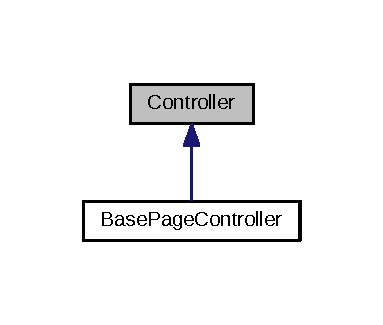
\includegraphics[width=184pt]{classController__inherit__graph}
\end{center}
\end{figure}
\subsection*{Public Member Functions}
\begin{DoxyCompactItemize}
\item 
\hyperlink{classController_ab91faf91a99b21a429324499f9ec9f70}{\+\_\+\+\_\+construct} (\$request)
\item 
\hyperlink{classController_a3057228d46eddceb352a1537ef05e8b7}{base\+Title} ()
\item 
\hyperlink{classController_a555247a38f8b4ea98a85bed7c6798e0a}{page\+Title} (\$page)
\item 
\hyperlink{classController_ae560b1221cb9f3891c432c3dd0292922}{set\+Title} (\$title)
\item 
\hyperlink{classController_af3f91509e2fbae1fd863df1577fcc4e7}{set\+Custom\+Title} (\$title)
\item 
\hyperlink{classController_ae8b4904843b2d665164620160b3c7157}{get\+Title} ()
\item 
\hyperlink{classController_aa844281accdd5aa2ca1ab1d890332b76}{get\+Page} ()
\item 
\hyperlink{classController_a90590c2cd8c1a89cc6eada64f0f24361}{safe\+Input} (\$input)
\item 
\hyperlink{classController_ac85206dce558e214f72fc3ca56f8cc31}{get\+Session\+Username} ()
\item 
\hyperlink{classController_a50e4138bea238a7bba318fffb948eeb1}{get\+Links} ()
\end{DoxyCompactItemize}
\subsection*{Public Attributes}
\begin{DoxyCompactItemize}
\item 
\hypertarget{classController_ae09902e0cf33dbffd52349e056794842}{{\bfseries \$request}}\label{classController_ae09902e0cf33dbffd52349e056794842}

\end{DoxyCompactItemize}
\subsection*{Protected Member Functions}
\begin{DoxyCompactItemize}
\item 
\hyperlink{classController_a014e1cea4dd7e6fb8fad83cdce9c6216}{is\+Logged\+In} ()
\item 
\hypertarget{classController_a5c1d8729360dbfe66bff62d7a60600d7}{{\bfseries is\+Admin} ()}\label{classController_a5c1d8729360dbfe66bff62d7a60600d7}

\item 
\hyperlink{classController_a67beb590eef4f36b07e6c9ef04fc8337}{close\+Session} ()
\end{DoxyCompactItemize}
\subsection*{Protected Attributes}
\begin{DoxyCompactItemize}
\item 
\hypertarget{classController_add0ea4a4a72b2f7cf707bdd435a67c61}{{\bfseries \$username}}\label{classController_add0ea4a4a72b2f7cf707bdd435a67c61}

\item 
\hypertarget{classController_a82584774d202d57e2e5159fa2add1079}{{\bfseries \$page}}\label{classController_a82584774d202d57e2e5159fa2add1079}

\end{DoxyCompactItemize}


\subsection{Detailed Description}
All controllers should inherit from here

\begin{DoxyAuthor}{Author}
fabio 
\end{DoxyAuthor}


\subsection{Constructor \& Destructor Documentation}
\hypertarget{classController_ab91faf91a99b21a429324499f9ec9f70}{\index{Controller@{Controller}!\+\_\+\+\_\+construct@{\+\_\+\+\_\+construct}}
\index{\+\_\+\+\_\+construct@{\+\_\+\+\_\+construct}!Controller@{Controller}}
\subsubsection[{\+\_\+\+\_\+construct}]{\setlength{\rightskip}{0pt plus 5cm}Controller\+::\+\_\+\+\_\+construct (
\begin{DoxyParamCaption}
\item[{}]{\$request}
\end{DoxyParamCaption}
)}}\label{classController_ab91faf91a99b21a429324499f9ec9f70}

\begin{DoxyParams}[1]{Parameters}
array & {\em \$request} & \\
\hline
\end{DoxyParams}


\subsection{Member Function Documentation}
\hypertarget{classController_a3057228d46eddceb352a1537ef05e8b7}{\index{Controller@{Controller}!base\+Title@{base\+Title}}
\index{base\+Title@{base\+Title}!Controller@{Controller}}
\subsubsection[{base\+Title}]{\setlength{\rightskip}{0pt plus 5cm}Controller\+::base\+Title (
\begin{DoxyParamCaption}
{}
\end{DoxyParamCaption}
)}}\label{classController_a3057228d46eddceb352a1537ef05e8b7}
\begin{DoxyReturn}{Returns}
string 
\end{DoxyReturn}
\hypertarget{classController_a67beb590eef4f36b07e6c9ef04fc8337}{\index{Controller@{Controller}!close\+Session@{close\+Session}}
\index{close\+Session@{close\+Session}!Controller@{Controller}}
\subsubsection[{close\+Session}]{\setlength{\rightskip}{0pt plus 5cm}Controller\+::close\+Session (
\begin{DoxyParamCaption}
{}
\end{DoxyParamCaption}
)\hspace{0.3cm}{\ttfamily [protected]}}}\label{classController_a67beb590eef4f36b07e6c9ef04fc8337}
Destroys the session. \hypertarget{classController_a50e4138bea238a7bba318fffb948eeb1}{\index{Controller@{Controller}!get\+Links@{get\+Links}}
\index{get\+Links@{get\+Links}!Controller@{Controller}}
\subsubsection[{get\+Links}]{\setlength{\rightskip}{0pt plus 5cm}Controller\+::get\+Links (
\begin{DoxyParamCaption}
{}
\end{DoxyParamCaption}
)}}\label{classController_a50e4138bea238a7bba318fffb948eeb1}
Returns a list of links. \hypertarget{classController_aa844281accdd5aa2ca1ab1d890332b76}{\index{Controller@{Controller}!get\+Page@{get\+Page}}
\index{get\+Page@{get\+Page}!Controller@{Controller}}
\subsubsection[{get\+Page}]{\setlength{\rightskip}{0pt plus 5cm}Controller\+::get\+Page (
\begin{DoxyParamCaption}
{}
\end{DoxyParamCaption}
)}}\label{classController_aa844281accdd5aa2ca1ab1d890332b76}
\begin{DoxyReturn}{Returns}
string 
\end{DoxyReturn}
\hypertarget{classController_ac85206dce558e214f72fc3ca56f8cc31}{\index{Controller@{Controller}!get\+Session\+Username@{get\+Session\+Username}}
\index{get\+Session\+Username@{get\+Session\+Username}!Controller@{Controller}}
\subsubsection[{get\+Session\+Username}]{\setlength{\rightskip}{0pt plus 5cm}Controller\+::get\+Session\+Username (
\begin{DoxyParamCaption}
{}
\end{DoxyParamCaption}
)}}\label{classController_ac85206dce558e214f72fc3ca56f8cc31}
Get the username saved in the session.

\begin{DoxyReturn}{Returns}
string 
\end{DoxyReturn}
\hypertarget{classController_ae8b4904843b2d665164620160b3c7157}{\index{Controller@{Controller}!get\+Title@{get\+Title}}
\index{get\+Title@{get\+Title}!Controller@{Controller}}
\subsubsection[{get\+Title}]{\setlength{\rightskip}{0pt plus 5cm}Controller\+::get\+Title (
\begin{DoxyParamCaption}
{}
\end{DoxyParamCaption}
)}}\label{classController_ae8b4904843b2d665164620160b3c7157}
\begin{DoxyReturn}{Returns}
string 
\end{DoxyReturn}
\hypertarget{classController_a014e1cea4dd7e6fb8fad83cdce9c6216}{\index{Controller@{Controller}!is\+Logged\+In@{is\+Logged\+In}}
\index{is\+Logged\+In@{is\+Logged\+In}!Controller@{Controller}}
\subsubsection[{is\+Logged\+In}]{\setlength{\rightskip}{0pt plus 5cm}Controller\+::is\+Logged\+In (
\begin{DoxyParamCaption}
{}
\end{DoxyParamCaption}
)\hspace{0.3cm}{\ttfamily [protected]}}}\label{classController_a014e1cea4dd7e6fb8fad83cdce9c6216}
Returns true if there's an active login session.

\begin{DoxyReturn}{Returns}
boolean 
\end{DoxyReturn}
\hypertarget{classController_a555247a38f8b4ea98a85bed7c6798e0a}{\index{Controller@{Controller}!page\+Title@{page\+Title}}
\index{page\+Title@{page\+Title}!Controller@{Controller}}
\subsubsection[{page\+Title}]{\setlength{\rightskip}{0pt plus 5cm}Controller\+::page\+Title (
\begin{DoxyParamCaption}
\item[{}]{\$page}
\end{DoxyParamCaption}
)}}\label{classController_a555247a38f8b4ea98a85bed7c6798e0a}

\begin{DoxyParams}[1]{Parameters}
array & {\em \$page} & \\
\hline
\end{DoxyParams}
\begin{DoxyReturn}{Returns}
string 
\end{DoxyReturn}
\hypertarget{classController_a90590c2cd8c1a89cc6eada64f0f24361}{\index{Controller@{Controller}!safe\+Input@{safe\+Input}}
\index{safe\+Input@{safe\+Input}!Controller@{Controller}}
\subsubsection[{safe\+Input}]{\setlength{\rightskip}{0pt plus 5cm}Controller\+::safe\+Input (
\begin{DoxyParamCaption}
\item[{}]{\$input}
\end{DoxyParamCaption}
)}}\label{classController_a90590c2cd8c1a89cc6eada64f0f24361}
Makes the input safe. 
\begin{DoxyParams}{Parameters}
{\em \$input} & string \\
\hline
\end{DoxyParams}
\begin{DoxyReturn}{Returns}
string 
\end{DoxyReturn}
\hypertarget{classController_af3f91509e2fbae1fd863df1577fcc4e7}{\index{Controller@{Controller}!set\+Custom\+Title@{set\+Custom\+Title}}
\index{set\+Custom\+Title@{set\+Custom\+Title}!Controller@{Controller}}
\subsubsection[{set\+Custom\+Title}]{\setlength{\rightskip}{0pt plus 5cm}Controller\+::set\+Custom\+Title (
\begin{DoxyParamCaption}
\item[{}]{\$title}
\end{DoxyParamCaption}
)}}\label{classController_af3f91509e2fbae1fd863df1577fcc4e7}

\begin{DoxyParams}[1]{Parameters}
string & {\em \$title} & \\
\hline
\end{DoxyParams}
\hypertarget{classController_ae560b1221cb9f3891c432c3dd0292922}{\index{Controller@{Controller}!set\+Title@{set\+Title}}
\index{set\+Title@{set\+Title}!Controller@{Controller}}
\subsubsection[{set\+Title}]{\setlength{\rightskip}{0pt plus 5cm}Controller\+::set\+Title (
\begin{DoxyParamCaption}
\item[{}]{\$title}
\end{DoxyParamCaption}
)}}\label{classController_ae560b1221cb9f3891c432c3dd0292922}

\begin{DoxyParams}[1]{Parameters}
string & {\em \$title} & \\
\hline
\end{DoxyParams}


The documentation for this class was generated from the following file\+:\begin{DoxyCompactItemize}
\item 
controller/Controller.\+php\end{DoxyCompactItemize}

\hypertarget{classDBModel}{\section{D\+B\+Model Class Reference}
\label{classDBModel}\index{D\+B\+Model@{D\+B\+Model}}
}


Inheritance diagram for D\+B\+Model\+:\nopagebreak
\begin{figure}[H]
\begin{center}
\leavevmode
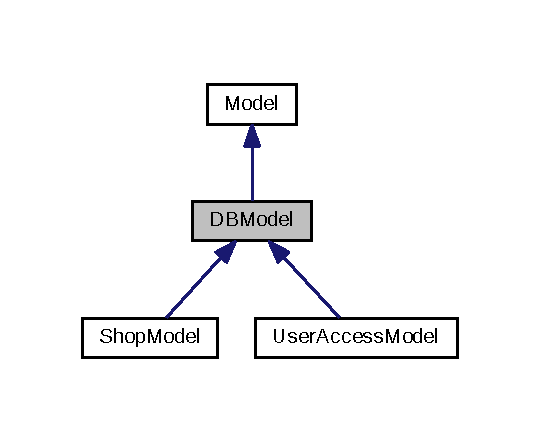
\includegraphics[width=259pt]{classDBModel__inherit__graph}
\end{center}
\end{figure}


Collaboration diagram for D\+B\+Model\+:\nopagebreak
\begin{figure}[H]
\begin{center}
\leavevmode
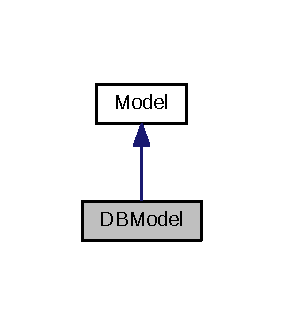
\includegraphics[width=136pt]{classDBModel__coll__graph}
\end{center}
\end{figure}
\subsection*{Protected Member Functions}
\begin{DoxyCompactItemize}
\item 
\hyperlink{classDBModel_af39102ef1235d8f2993208bc320ad0ce}{db\+Hostname} ()
\item 
\hyperlink{classDBModel_a8114bdda6fb2b260ce3c56710d0f9d1c}{db\+Database} ()
\item 
\hyperlink{classDBModel_a17aab9a5c0364118192c892e8dbd55f0}{db\+Username} ()
\item 
\hyperlink{classDBModel_a8596b488008a8b12a6dce706490fb68b}{db\+Password} ()
\item 
\hyperlink{classDBModel_ad54a4dc85f41f25cbf7675b712d5d5ff}{connect} ()
\end{DoxyCompactItemize}
\subsection*{Additional Inherited Members}


\subsection{Detailed Description}
Description of \hyperlink{classDBModel}{D\+B\+Model}.

\$dbhost = \char`\"{}localhost\char`\"{}; \$dbname = \char`\"{}amm15\+\_\+colella\+Fabio\char`\"{}; \$dbuser = \char`\"{}colella\+Fabio\char`\"{}; \$dbpass = \char`\"{}nutria8058\char`\"{};

\begin{DoxyAuthor}{Author}
fabio 
\end{DoxyAuthor}


\subsection{Member Function Documentation}
\hypertarget{classDBModel_ad54a4dc85f41f25cbf7675b712d5d5ff}{\index{D\+B\+Model@{D\+B\+Model}!connect@{connect}}
\index{connect@{connect}!D\+B\+Model@{D\+B\+Model}}
\subsubsection[{connect}]{\setlength{\rightskip}{0pt plus 5cm}D\+B\+Model\+::connect (
\begin{DoxyParamCaption}
{}
\end{DoxyParamCaption}
)\hspace{0.3cm}{\ttfamily [protected]}}}\label{classDBModel_ad54a4dc85f41f25cbf7675b712d5d5ff}
Create a connection.

If it fails connecting thrown an exception.

\begin{DoxyReturn}{Returns}
mysqli mysqli 
\end{DoxyReturn}
\hypertarget{classDBModel_a8114bdda6fb2b260ce3c56710d0f9d1c}{\index{D\+B\+Model@{D\+B\+Model}!db\+Database@{db\+Database}}
\index{db\+Database@{db\+Database}!D\+B\+Model@{D\+B\+Model}}
\subsubsection[{db\+Database}]{\setlength{\rightskip}{0pt plus 5cm}D\+B\+Model\+::db\+Database (
\begin{DoxyParamCaption}
{}
\end{DoxyParamCaption}
)\hspace{0.3cm}{\ttfamily [protected]}}}\label{classDBModel_a8114bdda6fb2b260ce3c56710d0f9d1c}
\begin{DoxyReturn}{Returns}
string database 
\end{DoxyReturn}
\hypertarget{classDBModel_af39102ef1235d8f2993208bc320ad0ce}{\index{D\+B\+Model@{D\+B\+Model}!db\+Hostname@{db\+Hostname}}
\index{db\+Hostname@{db\+Hostname}!D\+B\+Model@{D\+B\+Model}}
\subsubsection[{db\+Hostname}]{\setlength{\rightskip}{0pt plus 5cm}D\+B\+Model\+::db\+Hostname (
\begin{DoxyParamCaption}
{}
\end{DoxyParamCaption}
)\hspace{0.3cm}{\ttfamily [protected]}}}\label{classDBModel_af39102ef1235d8f2993208bc320ad0ce}
\begin{DoxyReturn}{Returns}
string hostname 
\end{DoxyReturn}
\hypertarget{classDBModel_a8596b488008a8b12a6dce706490fb68b}{\index{D\+B\+Model@{D\+B\+Model}!db\+Password@{db\+Password}}
\index{db\+Password@{db\+Password}!D\+B\+Model@{D\+B\+Model}}
\subsubsection[{db\+Password}]{\setlength{\rightskip}{0pt plus 5cm}D\+B\+Model\+::db\+Password (
\begin{DoxyParamCaption}
{}
\end{DoxyParamCaption}
)\hspace{0.3cm}{\ttfamily [protected]}}}\label{classDBModel_a8596b488008a8b12a6dce706490fb68b}
\begin{DoxyReturn}{Returns}
string password 
\end{DoxyReturn}
\hypertarget{classDBModel_a17aab9a5c0364118192c892e8dbd55f0}{\index{D\+B\+Model@{D\+B\+Model}!db\+Username@{db\+Username}}
\index{db\+Username@{db\+Username}!D\+B\+Model@{D\+B\+Model}}
\subsubsection[{db\+Username}]{\setlength{\rightskip}{0pt plus 5cm}D\+B\+Model\+::db\+Username (
\begin{DoxyParamCaption}
{}
\end{DoxyParamCaption}
)\hspace{0.3cm}{\ttfamily [protected]}}}\label{classDBModel_a17aab9a5c0364118192c892e8dbd55f0}
\begin{DoxyReturn}{Returns}
string username 
\end{DoxyReturn}


The documentation for this class was generated from the following file\+:\begin{DoxyCompactItemize}
\item 
model/D\+B\+Model.\+php\end{DoxyCompactItemize}

\hypertarget{classFooter}{\section{Footer Class Reference}
\label{classFooter}\index{Footer@{Footer}}
}


\subsection{Detailed Description}
Description of \hyperlink{classFooter}{Footer}

\begin{DoxyAuthor}{Author}
fabio 
\end{DoxyAuthor}


The documentation for this class was generated from the following file\+:\begin{DoxyCompactItemize}
\item 
view/Footer.\+php\end{DoxyCompactItemize}

\hypertarget{classForm}{\section{Form Class Reference}
\label{classForm}\index{Form@{Form}}
}
\subsection*{Public Member Functions}
\begin{DoxyCompactItemize}
\item 
\hyperlink{classForm_a3e3459dffd7067e2e707e0a622945a66}{get\+Signup\+Form} (\hyperlink{classUser}{User} \$user, \&\$error)
\item 
\hypertarget{classForm_a6a05f450eb73a3524602817c34da17be}{{\bfseries get\+Signup\+Confirmation} (\hyperlink{classUser}{User} \$user)}\label{classForm_a6a05f450eb73a3524602817c34da17be}

\item 
\hypertarget{classForm_a11a02f548641b39c9c7c04436c95befa}{{\bfseries get\+Signup\+Error\+Database} ()}\label{classForm_a11a02f548641b39c9c7c04436c95befa}

\item 
\hyperlink{classForm_aa3ff4d216868165f1f8c442ae7ea7c95}{get\+Login\+Form} (\$username, \&\$error)
\item 
\hyperlink{classForm_a61045a8ccfd7f300a729027a70a00700}{get\+Login\+Confirmation} (\$username)
\item 
\hyperlink{classForm_a08c23069323910390d5fc8d4ede9690d}{get\+Logout} (\$username)
\item 
\hyperlink{classForm_a9fe8a5c4812f4cbe0ff7daa05ea40cbf}{get\+Addshop\+Form} (\$data, \&\$error)
\item 
\hyperlink{classForm_a00d84099c9d0a8fd6cdc77983b2dac93}{get\+Addshop\+Confirmation} ()
\item 
\hyperlink{classForm_a12b1a6bb3a44baa1b311e8cc42759f9c}{generate\+Months\+Options} (\$selected=\char`\"{}\char`\"{})
\item 
\hyperlink{classForm_ae79e7e1de18f9f611d1e405349828104}{generate\+Days\+Options} (\$selected=\char`\"{}\char`\"{})
\item 
\hyperlink{classForm_a5bcd8bfb0770d2ca9e6874b329ab7f58}{generate\+Years\+Options} (\$selected=\char`\"{}\char`\"{})
\end{DoxyCompactItemize}


\subsection{Detailed Description}
\hyperlink{classForm}{Form} to sign up to the website. 

\subsection{Member Function Documentation}
\hypertarget{classForm_ae79e7e1de18f9f611d1e405349828104}{\index{Form@{Form}!generate\+Days\+Options@{generate\+Days\+Options}}
\index{generate\+Days\+Options@{generate\+Days\+Options}!Form@{Form}}
\subsubsection[{generate\+Days\+Options}]{\setlength{\rightskip}{0pt plus 5cm}Form\+::generate\+Days\+Options (
\begin{DoxyParamCaption}
\item[{}]{\$selected = {\ttfamily \char`\"{}\char`\"{}}}
\end{DoxyParamCaption}
)}}\label{classForm_ae79e7e1de18f9f611d1e405349828104}
Generates a days dropdown menu. 
\begin{DoxyParams}{Parameters}
{\em a} & default option \\
\hline
\end{DoxyParams}
\begin{DoxyReturn}{Returns}
string days\+Options 
\end{DoxyReturn}
\hypertarget{classForm_a12b1a6bb3a44baa1b311e8cc42759f9c}{\index{Form@{Form}!generate\+Months\+Options@{generate\+Months\+Options}}
\index{generate\+Months\+Options@{generate\+Months\+Options}!Form@{Form}}
\subsubsection[{generate\+Months\+Options}]{\setlength{\rightskip}{0pt plus 5cm}Form\+::generate\+Months\+Options (
\begin{DoxyParamCaption}
\item[{}]{\$selected = {\ttfamily \char`\"{}\char`\"{}}}
\end{DoxyParamCaption}
)}}\label{classForm_a12b1a6bb3a44baa1b311e8cc42759f9c}
Generates a months dropdown menu. 
\begin{DoxyParams}{Parameters}
{\em a} & default option \\
\hline
\end{DoxyParams}
\begin{DoxyReturn}{Returns}
string month\+Options 
\end{DoxyReturn}
\hypertarget{classForm_a5bcd8bfb0770d2ca9e6874b329ab7f58}{\index{Form@{Form}!generate\+Years\+Options@{generate\+Years\+Options}}
\index{generate\+Years\+Options@{generate\+Years\+Options}!Form@{Form}}
\subsubsection[{generate\+Years\+Options}]{\setlength{\rightskip}{0pt plus 5cm}Form\+::generate\+Years\+Options (
\begin{DoxyParamCaption}
\item[{}]{\$selected = {\ttfamily \char`\"{}\char`\"{}}}
\end{DoxyParamCaption}
)}}\label{classForm_a5bcd8bfb0770d2ca9e6874b329ab7f58}
Generates a years dropdown menu. 
\begin{DoxyParams}{Parameters}
{\em a} & default option \\
\hline
\end{DoxyParams}
\begin{DoxyReturn}{Returns}
string years\+Options 
\end{DoxyReturn}
\hypertarget{classForm_a00d84099c9d0a8fd6cdc77983b2dac93}{\index{Form@{Form}!get\+Addshop\+Confirmation@{get\+Addshop\+Confirmation}}
\index{get\+Addshop\+Confirmation@{get\+Addshop\+Confirmation}!Form@{Form}}
\subsubsection[{get\+Addshop\+Confirmation}]{\setlength{\rightskip}{0pt plus 5cm}Form\+::get\+Addshop\+Confirmation (
\begin{DoxyParamCaption}
{}
\end{DoxyParamCaption}
)}}\label{classForm_a00d84099c9d0a8fd6cdc77983b2dac93}
Create a login confirmation.


\begin{DoxyParams}[1]{Parameters}
string & {\em \$username} & \\
\hline
\end{DoxyParams}
\begin{DoxyReturn}{Returns}
string 
\end{DoxyReturn}
\hypertarget{classForm_a9fe8a5c4812f4cbe0ff7daa05ea40cbf}{\index{Form@{Form}!get\+Addshop\+Form@{get\+Addshop\+Form}}
\index{get\+Addshop\+Form@{get\+Addshop\+Form}!Form@{Form}}
\subsubsection[{get\+Addshop\+Form}]{\setlength{\rightskip}{0pt plus 5cm}Form\+::get\+Addshop\+Form (
\begin{DoxyParamCaption}
\item[{}]{\$data, }
\item[{\&}]{\$error}
\end{DoxyParamCaption}
)}}\label{classForm_a9fe8a5c4812f4cbe0ff7daa05ea40cbf}
Return a shop form.


\begin{DoxyParams}{Parameters}
{\em string\mbox{[}$\,$\mbox{]}\mbox{[}$\,$\mbox{]}} & \$data \\
\hline
{\em string\mbox{[}$\,$\mbox{]}} & \$error \\
\hline
\end{DoxyParams}
\begin{DoxyReturn}{Returns}
string 
\end{DoxyReturn}
\hypertarget{classForm_a61045a8ccfd7f300a729027a70a00700}{\index{Form@{Form}!get\+Login\+Confirmation@{get\+Login\+Confirmation}}
\index{get\+Login\+Confirmation@{get\+Login\+Confirmation}!Form@{Form}}
\subsubsection[{get\+Login\+Confirmation}]{\setlength{\rightskip}{0pt plus 5cm}Form\+::get\+Login\+Confirmation (
\begin{DoxyParamCaption}
\item[{}]{\$username}
\end{DoxyParamCaption}
)}}\label{classForm_a61045a8ccfd7f300a729027a70a00700}
Create a login confirmation.


\begin{DoxyParams}[1]{Parameters}
string & {\em \$username} & \\
\hline
\end{DoxyParams}
\begin{DoxyReturn}{Returns}
string 
\end{DoxyReturn}
\hypertarget{classForm_aa3ff4d216868165f1f8c442ae7ea7c95}{\index{Form@{Form}!get\+Login\+Form@{get\+Login\+Form}}
\index{get\+Login\+Form@{get\+Login\+Form}!Form@{Form}}
\subsubsection[{get\+Login\+Form}]{\setlength{\rightskip}{0pt plus 5cm}Form\+::get\+Login\+Form (
\begin{DoxyParamCaption}
\item[{}]{\$username, }
\item[{\&}]{\$error}
\end{DoxyParamCaption}
)}}\label{classForm_aa3ff4d216868165f1f8c442ae7ea7c95}
Login \hypertarget{classForm_a08c23069323910390d5fc8d4ede9690d}{\index{Form@{Form}!get\+Logout@{get\+Logout}}
\index{get\+Logout@{get\+Logout}!Form@{Form}}
\subsubsection[{get\+Logout}]{\setlength{\rightskip}{0pt plus 5cm}Form\+::get\+Logout (
\begin{DoxyParamCaption}
\item[{}]{\$username}
\end{DoxyParamCaption}
)}}\label{classForm_a08c23069323910390d5fc8d4ede9690d}
Logout \hypertarget{classForm_a3e3459dffd7067e2e707e0a622945a66}{\index{Form@{Form}!get\+Signup\+Form@{get\+Signup\+Form}}
\index{get\+Signup\+Form@{get\+Signup\+Form}!Form@{Form}}
\subsubsection[{get\+Signup\+Form}]{\setlength{\rightskip}{0pt plus 5cm}Form\+::get\+Signup\+Form (
\begin{DoxyParamCaption}
\item[{{\bf User}}]{\$user, }
\item[{\&}]{\$error}
\end{DoxyParamCaption}
)}}\label{classForm_a3e3459dffd7067e2e707e0a622945a66}
Signup Set the latest choices for the date fields 

The documentation for this class was generated from the following file\+:\begin{DoxyCompactItemize}
\item 
view/Form.\+php\end{DoxyCompactItemize}

\hypertarget{classGenericModel}{\section{Generic\+Model Class Reference}
\label{classGenericModel}\index{Generic\+Model@{Generic\+Model}}
}


Inheritance diagram for Generic\+Model\+:\nopagebreak
\begin{figure}[H]
\begin{center}
\leavevmode
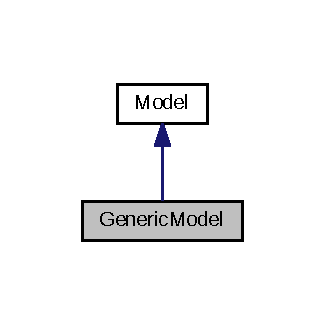
\includegraphics[width=156pt]{classGenericModel__inherit__graph}
\end{center}
\end{figure}


Collaboration diagram for Generic\+Model\+:\nopagebreak
\begin{figure}[H]
\begin{center}
\leavevmode
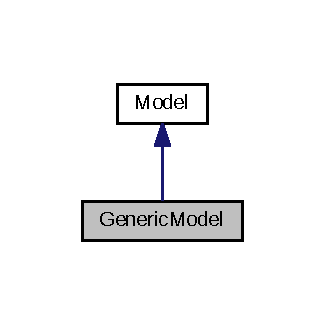
\includegraphics[width=156pt]{classGenericModel__coll__graph}
\end{center}
\end{figure}
\subsection*{Public Member Functions}
\begin{DoxyCompactItemize}
\item 
\hypertarget{classGenericModel_acd2ddd6efe0003c9fe876517307bf7d4}{{\bfseries \+\_\+\+\_\+construct} (\$request)}\label{classGenericModel_acd2ddd6efe0003c9fe876517307bf7d4}

\item 
\hyperlink{classGenericModel_a1fea07f39a9346955dff26476dac4650}{show} ()
\item 
\hyperlink{classGenericModel_acd7009f2fcaca1b046b371fe23e0fd2c}{show\+Help\+Page} ()
\end{DoxyCompactItemize}
\subsection*{Additional Inherited Members}


\subsection{Detailed Description}
This is a generic model class. Extend it if you're doing very simple pages that don't require a specific model. 

\subsection{Member Function Documentation}
\hypertarget{classGenericModel_a1fea07f39a9346955dff26476dac4650}{\index{Generic\+Model@{Generic\+Model}!show@{show}}
\index{show@{show}!Generic\+Model@{Generic\+Model}}
\subsubsection[{show}]{\setlength{\rightskip}{0pt plus 5cm}Generic\+Model\+::show (
\begin{DoxyParamCaption}
{}
\end{DoxyParamCaption}
)}}\label{classGenericModel_a1fea07f39a9346955dff26476dac4650}
This function is required by the model. \hypertarget{classGenericModel_acd7009f2fcaca1b046b371fe23e0fd2c}{\index{Generic\+Model@{Generic\+Model}!show\+Help\+Page@{show\+Help\+Page}}
\index{show\+Help\+Page@{show\+Help\+Page}!Generic\+Model@{Generic\+Model}}
\subsubsection[{show\+Help\+Page}]{\setlength{\rightskip}{0pt plus 5cm}Generic\+Model\+::show\+Help\+Page (
\begin{DoxyParamCaption}
{}
\end{DoxyParamCaption}
)}}\label{classGenericModel_acd7009f2fcaca1b046b371fe23e0fd2c}
Handles the help page. 

The documentation for this class was generated from the following file\+:\begin{DoxyCompactItemize}
\item 
model/Generic\+Model.\+php\end{DoxyCompactItemize}

\hypertarget{classGenericView}{\section{Generic\+View Class Reference}
\label{classGenericView}\index{Generic\+View@{Generic\+View}}
}
\subsection*{Public Member Functions}
\begin{DoxyCompactItemize}
\item 
\hyperlink{classGenericView_af4707380a714031af8a721909dcc588f}{get\+Profile\+View} (\$user)
\item 
\hypertarget{classGenericView_a0901126944127bdad1bdea93f37bfb1b}{{\bfseries get\+Home\+Content} (\$data)}\label{classGenericView_a0901126944127bdad1bdea93f37bfb1b}

\end{DoxyCompactItemize}


\subsection{Member Function Documentation}
\hypertarget{classGenericView_af4707380a714031af8a721909dcc588f}{\index{Generic\+View@{Generic\+View}!get\+Profile\+View@{get\+Profile\+View}}
\index{get\+Profile\+View@{get\+Profile\+View}!Generic\+View@{Generic\+View}}
\subsubsection[{get\+Profile\+View}]{\setlength{\rightskip}{0pt plus 5cm}Generic\+View\+::get\+Profile\+View (
\begin{DoxyParamCaption}
\item[{}]{\$user}
\end{DoxyParamCaption}
)}}\label{classGenericView_af4707380a714031af8a721909dcc588f}
Get the H\+T\+M\+L to render the profile.


\begin{DoxyParams}{Parameters}
{\em profile} & string\mbox{[}\mbox{]} \\
\hline
\end{DoxyParams}
\begin{DoxyReturn}{Returns}
string H\+T\+M\+L view 
\end{DoxyReturn}


The documentation for this class was generated from the following file\+:\begin{DoxyCompactItemize}
\item 
view/Generic\+Views.\+php\end{DoxyCompactItemize}

\hypertarget{classHead}{\section{Head Class Reference}
\label{classHead}\index{Head@{Head}}
}
\subsection*{Public Member Functions}
\begin{DoxyCompactItemize}
\item 
\hypertarget{classHead_a27eca7d61c333ac734cfc1d65b928b03}{{\bfseries \+\_\+\+\_\+construct} (\$title, \$fields=\char`\"{}\char`\"{})}\label{classHead_a27eca7d61c333ac734cfc1d65b928b03}

\end{DoxyCompactItemize}


\subsection{Detailed Description}
Description of head

\begin{DoxyAuthor}{Author}
fabio 
\end{DoxyAuthor}


The documentation for this class was generated from the following file\+:\begin{DoxyCompactItemize}
\item 
view/Head.\+php\end{DoxyCompactItemize}

\hypertarget{classHeader}{\section{Header Class Reference}
\label{classHeader}\index{Header@{Header}}
}


\subsection{Detailed Description}
Description of \hyperlink{classHeader}{Header}

\begin{DoxyAuthor}{Author}
fabio 
\end{DoxyAuthor}


The documentation for this class was generated from the following file\+:\begin{DoxyCompactItemize}
\item 
view/Header.\+php\end{DoxyCompactItemize}

\hypertarget{classHomeModel}{\section{Home\+Model Class Reference}
\label{classHomeModel}\index{Home\+Model@{Home\+Model}}
}


Inheritance diagram for Home\+Model\+:\nopagebreak
\begin{figure}[H]
\begin{center}
\leavevmode
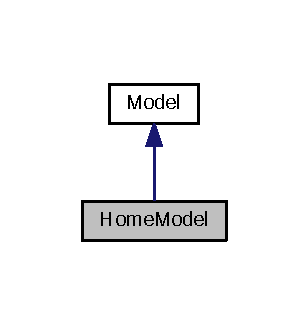
\includegraphics[width=148pt]{classHomeModel__inherit__graph}
\end{center}
\end{figure}


Collaboration diagram for Home\+Model\+:\nopagebreak
\begin{figure}[H]
\begin{center}
\leavevmode
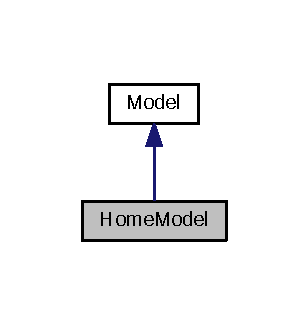
\includegraphics[width=148pt]{classHomeModel__coll__graph}
\end{center}
\end{figure}
\subsection*{Additional Inherited Members}


\subsection{Detailed Description}
Description of \hyperlink{classHomeModel}{Home\+Model}

\begin{DoxyAuthor}{Author}
Fabio Colella 
\end{DoxyAuthor}


The documentation for this class was generated from the following file\+:\begin{DoxyCompactItemize}
\item 
model/Home\+Model.\+php\end{DoxyCompactItemize}

\hypertarget{classModel}{\section{Model Class Reference}
\label{classModel}\index{Model@{Model}}
}


Inheritance diagram for Model\+:\nopagebreak
\begin{figure}[H]
\begin{center}
\leavevmode
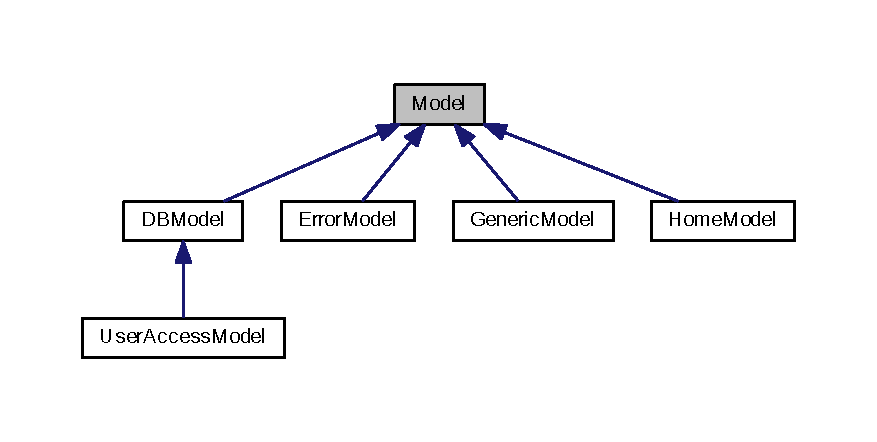
\includegraphics[width=350pt]{classModel__inherit__graph}
\end{center}
\end{figure}
\subsection*{Public Member Functions}
\begin{DoxyCompactItemize}
\item 
\hyperlink{classModel_a655d64396144aad24a62132fa11b92ea}{\+\_\+\+\_\+construct} ()
\item 
\hyperlink{classModel_af422ec4a1428678240da4e751f942b9c}{add\+Data} (\$name, \$data)
\item 
\hyperlink{classModel_a8e1cba2731a082294561ce1b499f3402}{get\+Data} (\$name)
\item 
\hyperlink{classModel_a0372eec1043cef6e9b6a50220cb0b031}{get\+Error} ()
\end{DoxyCompactItemize}
\subsection*{Protected Attributes}
\begin{DoxyCompactItemize}
\item 
\hypertarget{classModel_ae04c729239482d90601ba5c9d6a4fc66}{{\bfseries \$data}}\label{classModel_ae04c729239482d90601ba5c9d6a4fc66}

\item 
\hypertarget{classModel_a4c02091587027b71fed8b3ff0a96748b}{{\bfseries \$error}}\label{classModel_a4c02091587027b71fed8b3ff0a96748b}

\end{DoxyCompactItemize}


\subsection{Detailed Description}
Collects methods and properties useful in every model.

\begin{DoxyAuthor}{Author}
Fabio Colella 
\end{DoxyAuthor}


\subsection{Constructor \& Destructor Documentation}
\hypertarget{classModel_a655d64396144aad24a62132fa11b92ea}{\index{Model@{Model}!\+\_\+\+\_\+construct@{\+\_\+\+\_\+construct}}
\index{\+\_\+\+\_\+construct@{\+\_\+\+\_\+construct}!Model@{Model}}
\subsubsection[{\+\_\+\+\_\+construct}]{\setlength{\rightskip}{0pt plus 5cm}Model\+::\+\_\+\+\_\+construct (
\begin{DoxyParamCaption}
{}
\end{DoxyParamCaption}
)}}\label{classModel_a655d64396144aad24a62132fa11b92ea}
The constructor. 

\subsection{Member Function Documentation}
\hypertarget{classModel_af422ec4a1428678240da4e751f942b9c}{\index{Model@{Model}!add\+Data@{add\+Data}}
\index{add\+Data@{add\+Data}!Model@{Model}}
\subsubsection[{add\+Data}]{\setlength{\rightskip}{0pt plus 5cm}Model\+::add\+Data (
\begin{DoxyParamCaption}
\item[{}]{\$name, }
\item[{}]{\$data}
\end{DoxyParamCaption}
)}}\label{classModel_af422ec4a1428678240da4e751f942b9c}
Add data to the associtive array.


\begin{DoxyParams}[1]{Parameters}
string & {\em \$name} & \\
\hline
mixed & {\em \$data} & \\
\hline
\end{DoxyParams}
\begin{DoxyReturn}{Returns}
boolean task\+Succeded 
\end{DoxyReturn}
\hypertarget{classModel_a8e1cba2731a082294561ce1b499f3402}{\index{Model@{Model}!get\+Data@{get\+Data}}
\index{get\+Data@{get\+Data}!Model@{Model}}
\subsubsection[{get\+Data}]{\setlength{\rightskip}{0pt plus 5cm}Model\+::get\+Data (
\begin{DoxyParamCaption}
\item[{}]{\$name}
\end{DoxyParamCaption}
)}}\label{classModel_a8e1cba2731a082294561ce1b499f3402}
Retrieve data from the associative array.


\begin{DoxyParams}[1]{Parameters}
string & {\em \$name} & \\
\hline
\end{DoxyParams}
\begin{DoxyReturn}{Returns}
mixed if data\mbox{[}\$name\mbox{]} is not present returns null. 
\end{DoxyReturn}
\hypertarget{classModel_a0372eec1043cef6e9b6a50220cb0b031}{\index{Model@{Model}!get\+Error@{get\+Error}}
\index{get\+Error@{get\+Error}!Model@{Model}}
\subsubsection[{get\+Error}]{\setlength{\rightskip}{0pt plus 5cm}Model\+::get\+Error (
\begin{DoxyParamCaption}
{}
\end{DoxyParamCaption}
)}}\label{classModel_a0372eec1043cef6e9b6a50220cb0b031}
Returns the error array.

\begin{DoxyReturn}{Returns}
array 
\end{DoxyReturn}


The documentation for this class was generated from the following file\+:\begin{DoxyCompactItemize}
\item 
model/Model.\+php\end{DoxyCompactItemize}

\hypertarget{classNav}{\section{Nav Class Reference}
\label{classNav}\index{Nav@{Nav}}
}
\subsection*{Public Member Functions}
\begin{DoxyCompactItemize}
\item 
\hypertarget{classNav_a7259952c17df9af4f7fef4bfce0c47a3}{{\bfseries \+\_\+\+\_\+construct} (\$other\+Links=null)}\label{classNav_a7259952c17df9af4f7fef4bfce0c47a3}

\item 
\hypertarget{classNav_a3e7c5d2f40a243aa27bcef340cf2ec9d}{{\bfseries render} ()}\label{classNav_a3e7c5d2f40a243aa27bcef340cf2ec9d}

\end{DoxyCompactItemize}


\subsection{Detailed Description}
Description of \hyperlink{classNav}{Nav}

\begin{DoxyAuthor}{Author}
fabio 
\end{DoxyAuthor}


The documentation for this class was generated from the following file\+:\begin{DoxyCompactItemize}
\item 
view/Nav.\+php\end{DoxyCompactItemize}

\hypertarget{classPresenter}{\section{Presenter Class Reference}
\label{classPresenter}\index{Presenter@{Presenter}}
}
\subsection*{Public Member Functions}
\begin{DoxyCompactItemize}
\item 
\hyperlink{classPresenter_a24c04a54ce929bc12219f037a794d439}{\+\_\+\+\_\+construct} (\$title, \$content=\char`\"{}\char`\"{})
\item 
\hypertarget{classPresenter_a299e31916fc252227e369fc5efad77f9}{{\bfseries set\+Custom\+Header} (\$header)}\label{classPresenter_a299e31916fc252227e369fc5efad77f9}

\item 
\hyperlink{classPresenter_a327ab1b725813be28114753935b42cd4}{print\+Content} (\$content, \$indentation= ' ')
\item 
\hyperlink{classPresenter_a8a9d11db6633e0ebb898abd4580f8988}{get\+Content} ()
\item 
\hyperlink{classPresenter_a9a7d0d294934548d13620baca0657087}{set\+Content} (\$content)
\item 
\hyperlink{classPresenter_a2194a46cf6c23dd4e483f1ee63bc2236}{render} ()
\item 
\hyperlink{classPresenter_a1d66815ed950c7362a9c87bbcc6d9b7b}{set\+Error} (\$error\+Array=array())
\item 
\hyperlink{classPresenter_a5e4fe61038c5535719c6d7bc3b557019}{print\+Error\+List} ()
\item 
\hyperlink{classPresenter_a517ff93f6c099065a0d67c0994f0b76b}{set\+Redir} (\$link=\char`\"{}index\char`\"{}, \$sec=3)
\item 
\hypertarget{classPresenter_ace2a8a72ee53e6be953614d00e29f741}{{\bfseries print\+Redir} ()}\label{classPresenter_ace2a8a72ee53e6be953614d00e29f741}

\end{DoxyCompactItemize}


\subsection{Detailed Description}
Describes the whole view and renders the page.

\begin{DoxyAuthor}{Author}
fabio 
\end{DoxyAuthor}


\subsection{Constructor \& Destructor Documentation}
\hypertarget{classPresenter_a24c04a54ce929bc12219f037a794d439}{\index{Presenter@{Presenter}!\+\_\+\+\_\+construct@{\+\_\+\+\_\+construct}}
\index{\+\_\+\+\_\+construct@{\+\_\+\+\_\+construct}!Presenter@{Presenter}}
\subsubsection[{\+\_\+\+\_\+construct}]{\setlength{\rightskip}{0pt plus 5cm}Presenter\+::\+\_\+\+\_\+construct (
\begin{DoxyParamCaption}
\item[{}]{\$title, }
\item[{}]{\$content = {\ttfamily \char`\"{}\char`\"{}}}
\end{DoxyParamCaption}
)}}\label{classPresenter_a24c04a54ce929bc12219f037a794d439}
View constructor.


\begin{DoxyParams}[1]{Parameters}
string & {\em \$title} & of the page \\
\hline
string & {\em \$content} & of the page \\
\hline
\end{DoxyParams}


\subsection{Member Function Documentation}
\hypertarget{classPresenter_a8a9d11db6633e0ebb898abd4580f8988}{\index{Presenter@{Presenter}!get\+Content@{get\+Content}}
\index{get\+Content@{get\+Content}!Presenter@{Presenter}}
\subsubsection[{get\+Content}]{\setlength{\rightskip}{0pt plus 5cm}Presenter\+::get\+Content (
\begin{DoxyParamCaption}
{}
\end{DoxyParamCaption}
)}}\label{classPresenter_a8a9d11db6633e0ebb898abd4580f8988}
Return some content to render.

\begin{DoxyReturn}{Returns}
string H\+T\+M\+L content. 
\end{DoxyReturn}
\hypertarget{classPresenter_a327ab1b725813be28114753935b42cd4}{\index{Presenter@{Presenter}!print\+Content@{print\+Content}}
\index{print\+Content@{print\+Content}!Presenter@{Presenter}}
\subsubsection[{print\+Content}]{\setlength{\rightskip}{0pt plus 5cm}Presenter\+::print\+Content (
\begin{DoxyParamCaption}
\item[{}]{\$content, }
\item[{}]{\$indentation = {\ttfamily '~~~~~~'}}
\end{DoxyParamCaption}
)}}\label{classPresenter_a327ab1b725813be28114753935b42cd4}
Prints the H\+T\+M\+L indented correctly.


\begin{DoxyParams}[1]{Parameters}
string & {\em \$content} & multiline \\
\hline
string & {\em \$indentation} & spaces indentation \\
\hline
\end{DoxyParams}
\hypertarget{classPresenter_a5e4fe61038c5535719c6d7bc3b557019}{\index{Presenter@{Presenter}!print\+Error\+List@{print\+Error\+List}}
\index{print\+Error\+List@{print\+Error\+List}!Presenter@{Presenter}}
\subsubsection[{print\+Error\+List}]{\setlength{\rightskip}{0pt plus 5cm}Presenter\+::print\+Error\+List (
\begin{DoxyParamCaption}
{}
\end{DoxyParamCaption}
)}}\label{classPresenter_a5e4fe61038c5535719c6d7bc3b557019}
Returns the H\+T\+M\+L code of the error list. \begin{DoxyReturn}{Returns}
string 
\end{DoxyReturn}
\hypertarget{classPresenter_a2194a46cf6c23dd4e483f1ee63bc2236}{\index{Presenter@{Presenter}!render@{render}}
\index{render@{render}!Presenter@{Presenter}}
\subsubsection[{render}]{\setlength{\rightskip}{0pt plus 5cm}Presenter\+::render (
\begin{DoxyParamCaption}
{}
\end{DoxyParamCaption}
)}}\label{classPresenter_a2194a46cf6c23dd4e483f1ee63bc2236}
Render the page \hypertarget{classPresenter_a9a7d0d294934548d13620baca0657087}{\index{Presenter@{Presenter}!set\+Content@{set\+Content}}
\index{set\+Content@{set\+Content}!Presenter@{Presenter}}
\subsubsection[{set\+Content}]{\setlength{\rightskip}{0pt plus 5cm}Presenter\+::set\+Content (
\begin{DoxyParamCaption}
\item[{}]{\$content}
\end{DoxyParamCaption}
)}}\label{classPresenter_a9a7d0d294934548d13620baca0657087}
Receive some content to render.


\begin{DoxyParams}[1]{Parameters}
string & {\em \$content} & H\+T\+M\+L content. \\
\hline
\end{DoxyParams}
\hypertarget{classPresenter_a1d66815ed950c7362a9c87bbcc6d9b7b}{\index{Presenter@{Presenter}!set\+Error@{set\+Error}}
\index{set\+Error@{set\+Error}!Presenter@{Presenter}}
\subsubsection[{set\+Error}]{\setlength{\rightskip}{0pt plus 5cm}Presenter\+::set\+Error (
\begin{DoxyParamCaption}
\item[{}]{\$error\+Array = {\ttfamily array()}}
\end{DoxyParamCaption}
)}}\label{classPresenter_a1d66815ed950c7362a9c87bbcc6d9b7b}
Sets the error list. 
\begin{DoxyParams}{Parameters}
{\em string\mbox{[}$\,$\mbox{]}} & \$error\+Array \\
\hline
\end{DoxyParams}
\hypertarget{classPresenter_a517ff93f6c099065a0d67c0994f0b76b}{\index{Presenter@{Presenter}!set\+Redir@{set\+Redir}}
\index{set\+Redir@{set\+Redir}!Presenter@{Presenter}}
\subsubsection[{set\+Redir}]{\setlength{\rightskip}{0pt plus 5cm}Presenter\+::set\+Redir (
\begin{DoxyParamCaption}
\item[{}]{\$link = {\ttfamily \char`\"{}index\char`\"{}}, }
\item[{}]{\$sec = {\ttfamily 3}}
\end{DoxyParamCaption}
)}}\label{classPresenter_a517ff93f6c099065a0d67c0994f0b76b}

\begin{DoxyParams}[1]{Parameters}
type & {\em \$link} & \\
\hline
\end{DoxyParams}


The documentation for this class was generated from the following file\+:\begin{DoxyCompactItemize}
\item 
view/Presenter.\+php\end{DoxyCompactItemize}

\hypertarget{classShopModel}{\section{Shop\+Model Class Reference}
\label{classShopModel}\index{Shop\+Model@{Shop\+Model}}
}


Inheritance diagram for Shop\+Model\+:\nopagebreak
\begin{figure}[H]
\begin{center}
\leavevmode
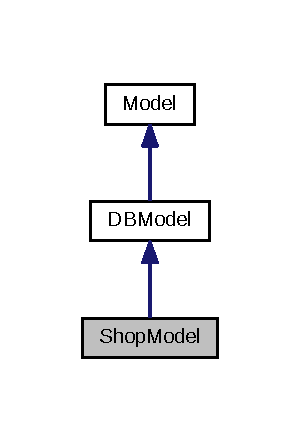
\includegraphics[width=144pt]{classShopModel__inherit__graph}
\end{center}
\end{figure}


Collaboration diagram for Shop\+Model\+:\nopagebreak
\begin{figure}[H]
\begin{center}
\leavevmode
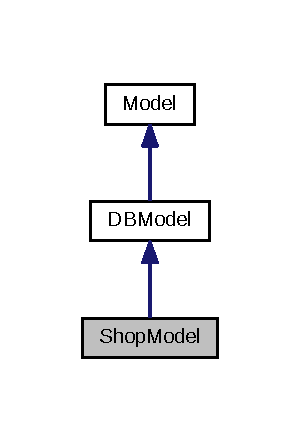
\includegraphics[width=144pt]{classShopModel__coll__graph}
\end{center}
\end{figure}
\subsection*{Public Member Functions}
\begin{DoxyCompactItemize}
\item 
\hyperlink{classShopModel_a67653f592dcfd15e7c3e8a0262fb824b}{add\+Shop\+To\+Database} (\$data)
\item 
\hyperlink{classShopModel_a5c5c4b2e0ea0e4adb98e6e6dea5011b6}{get\+Data} (\$search=\char`\"{}\char`\"{})
\item 
\hyperlink{classShopModel_ae035aa872e97c08247d203f90e228fe2}{remove\+Shop} (\$shop\+\_\+name, \$id)
\end{DoxyCompactItemize}
\subsection*{Additional Inherited Members}


\subsection{Detailed Description}
Description of shop\+Model

\begin{DoxyAuthor}{Author}
fabio 
\end{DoxyAuthor}


\subsection{Member Function Documentation}
\hypertarget{classShopModel_a67653f592dcfd15e7c3e8a0262fb824b}{\index{Shop\+Model@{Shop\+Model}!add\+Shop\+To\+Database@{add\+Shop\+To\+Database}}
\index{add\+Shop\+To\+Database@{add\+Shop\+To\+Database}!Shop\+Model@{Shop\+Model}}
\subsubsection[{add\+Shop\+To\+Database}]{\setlength{\rightskip}{0pt plus 5cm}Shop\+Model\+::add\+Shop\+To\+Database (
\begin{DoxyParamCaption}
\item[{}]{\$data}
\end{DoxyParamCaption}
)}}\label{classShopModel_a67653f592dcfd15e7c3e8a0262fb824b}
Remove unsetted values from submission \hypertarget{classShopModel_a5c5c4b2e0ea0e4adb98e6e6dea5011b6}{\index{Shop\+Model@{Shop\+Model}!get\+Data@{get\+Data}}
\index{get\+Data@{get\+Data}!Shop\+Model@{Shop\+Model}}
\subsubsection[{get\+Data}]{\setlength{\rightskip}{0pt plus 5cm}Shop\+Model\+::get\+Data (
\begin{DoxyParamCaption}
\item[{}]{\$search = {\ttfamily \char`\"{}\char`\"{}}}
\end{DoxyParamCaption}
)}}\label{classShopModel_a5c5c4b2e0ea0e4adb98e6e6dea5011b6}
Retrieve the shop data from the database.


\begin{DoxyParams}[1]{Parameters}
string & {\em \$search} & \\
\hline
\end{DoxyParams}
\begin{DoxyReturn}{Returns}
string\mbox{[}\mbox{]}\mbox{[}\mbox{]} 
\end{DoxyReturn}
\hypertarget{classShopModel_ae035aa872e97c08247d203f90e228fe2}{\index{Shop\+Model@{Shop\+Model}!remove\+Shop@{remove\+Shop}}
\index{remove\+Shop@{remove\+Shop}!Shop\+Model@{Shop\+Model}}
\subsubsection[{remove\+Shop}]{\setlength{\rightskip}{0pt plus 5cm}Shop\+Model\+::remove\+Shop (
\begin{DoxyParamCaption}
\item[{}]{\$shop\+\_\+name, }
\item[{}]{\$id}
\end{DoxyParamCaption}
)}}\label{classShopModel_ae035aa872e97c08247d203f90e228fe2}
Delete a shop data from the database.


\begin{DoxyParams}[1]{Parameters}
string & {\em \$search} & \\
\hline
\end{DoxyParams}
\begin{DoxyReturn}{Returns}
string\mbox{[}\mbox{]}\mbox{[}\mbox{]} 
\end{DoxyReturn}


The documentation for this class was generated from the following file\+:\begin{DoxyCompactItemize}
\item 
model/Shop\+Model.\+php\end{DoxyCompactItemize}

\hypertarget{classUser}{\section{User Class Reference}
\label{classUser}\index{User@{User}}
}
\subsection*{Public Member Functions}
\begin{DoxyCompactItemize}
\item 
\hyperlink{classUser_a06c940ee40777907844d9bd01ed20e2f}{field\+List} ()
\item 
\hyperlink{classUser_a3e0d1d6040692cac64fa423f21d50fa9}{\+\_\+\+\_\+construct} (\$firstname=\char`\"{}\char`\"{}, \$secondname=\char`\"{}\char`\"{}, \$email=\char`\"{}\char`\"{}, \$username=\char`\"{}\char`\"{}, \$password=\char`\"{}\char`\"{}, \$birthdate=\char`\"{}\char`\"{}, \$is\+Admin=false, \$confirmed=false)
\item 
\hyperlink{classUser_ac3880c17324e5d182bae56655365df85}{get} (\$field)
\item 
\hyperlink{classUser_af9023f37771e314acc0707060a449bb8}{set} (\$field, \$value)
\end{DoxyCompactItemize}


\subsection{Detailed Description}
This class defines an object used to represent a user and its properties.

\begin{DoxyAuthor}{Author}
Fabio Colella 
\end{DoxyAuthor}


\subsection{Constructor \& Destructor Documentation}
\hypertarget{classUser_a3e0d1d6040692cac64fa423f21d50fa9}{\index{User@{User}!\+\_\+\+\_\+construct@{\+\_\+\+\_\+construct}}
\index{\+\_\+\+\_\+construct@{\+\_\+\+\_\+construct}!User@{User}}
\subsubsection[{\+\_\+\+\_\+construct}]{\setlength{\rightskip}{0pt plus 5cm}User\+::\+\_\+\+\_\+construct (
\begin{DoxyParamCaption}
\item[{}]{\$firstname = {\ttfamily \char`\"{}\char`\"{}}, }
\item[{}]{\$secondname = {\ttfamily \char`\"{}\char`\"{}}, }
\item[{}]{\$email = {\ttfamily \char`\"{}\char`\"{}}, }
\item[{}]{\$username = {\ttfamily \char`\"{}\char`\"{}}, }
\item[{}]{\$password = {\ttfamily \char`\"{}\char`\"{}}, }
\item[{}]{\$birthdate = {\ttfamily \char`\"{}\char`\"{}}, }
\item[{}]{\$is\+Admin = {\ttfamily false}, }
\item[{}]{\$confirmed = {\ttfamily false}}
\end{DoxyParamCaption}
)}}\label{classUser_a3e0d1d6040692cac64fa423f21d50fa9}
The constructor.


\begin{DoxyParams}[1]{Parameters}
string & {\em \$firstname} & the firstname. \\
\hline
string & {\em \$secondname} & the secondname. \\
\hline
string & {\em \$email} & the email. \\
\hline
string & {\em \$username} & the username. \\
\hline
string & {\em \$password} & the password. \\
\hline
string & {\em \$birthdate} & the birthday in format Y\+Y\+Y\+Y-\/\+M\+M-\/\+D\+D. \\
\hline
boolean & {\em \$is\+Admin} & true if is admin. \\
\hline
boolean & {\em \$confirmed} & true if is a confirmed user. \\
\hline
\end{DoxyParams}


\subsection{Member Function Documentation}
\hypertarget{classUser_a06c940ee40777907844d9bd01ed20e2f}{\index{User@{User}!field\+List@{field\+List}}
\index{field\+List@{field\+List}!User@{User}}
\subsubsection[{field\+List}]{\setlength{\rightskip}{0pt plus 5cm}User\+::field\+List (
\begin{DoxyParamCaption}
{}
\end{DoxyParamCaption}
)}}\label{classUser_a06c940ee40777907844d9bd01ed20e2f}
Returns a list of the fields.

\begin{DoxyReturn}{Returns}
array list of field names. 
\end{DoxyReturn}
\hypertarget{classUser_ac3880c17324e5d182bae56655365df85}{\index{User@{User}!get@{get}}
\index{get@{get}!User@{User}}
\subsubsection[{get}]{\setlength{\rightskip}{0pt plus 5cm}User\+::get (
\begin{DoxyParamCaption}
\item[{}]{\$field}
\end{DoxyParamCaption}
)}}\label{classUser_ac3880c17324e5d182bae56655365df85}
Get a field value.


\begin{DoxyParams}[1]{Parameters}
string & {\em \$field} & the field name. \\
\hline
\end{DoxyParams}
\begin{DoxyReturn}{Returns}
mixed the value of the field. 
\end{DoxyReturn}
\hypertarget{classUser_af9023f37771e314acc0707060a449bb8}{\index{User@{User}!set@{set}}
\index{set@{set}!User@{User}}
\subsubsection[{set}]{\setlength{\rightskip}{0pt plus 5cm}User\+::set (
\begin{DoxyParamCaption}
\item[{}]{\$field, }
\item[{}]{\$value}
\end{DoxyParamCaption}
)}}\label{classUser_af9023f37771e314acc0707060a449bb8}
Sets a value for a field.


\begin{DoxyParams}[1]{Parameters}
string & {\em \$field} & the field name. \\
\hline
mixed & {\em \$value} & the value to set. \\
\hline
\end{DoxyParams}


The documentation for this class was generated from the following file\+:\begin{DoxyCompactItemize}
\item 
model/User.\+php\end{DoxyCompactItemize}

\hypertarget{classUserAccessModel}{\section{User\+Access\+Model Class Reference}
\label{classUserAccessModel}\index{User\+Access\+Model@{User\+Access\+Model}}
}


Inheritance diagram for User\+Access\+Model\+:\nopagebreak
\begin{figure}[H]
\begin{center}
\leavevmode
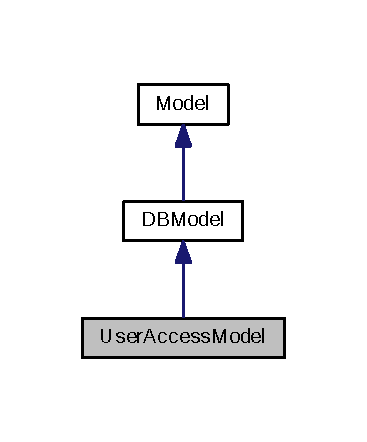
\includegraphics[width=176pt]{classUserAccessModel__inherit__graph}
\end{center}
\end{figure}


Collaboration diagram for User\+Access\+Model\+:\nopagebreak
\begin{figure}[H]
\begin{center}
\leavevmode
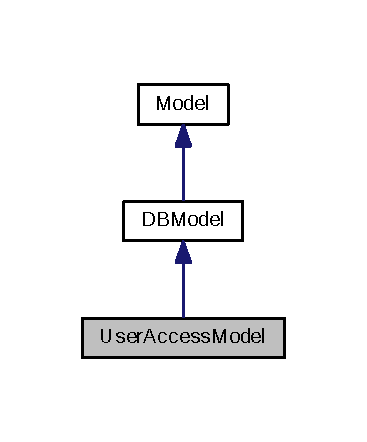
\includegraphics[width=176pt]{classUserAccessModel__coll__graph}
\end{center}
\end{figure}
\subsection*{Public Member Functions}
\begin{DoxyCompactItemize}
\item 
\hyperlink{classUserAccessModel_a4ff78b6bca940216de17457d8ec7f76d}{\+\_\+\+\_\+construct} ()
\item 
\hyperlink{classUserAccessModel_a65363d66e0dcf1cdf7caea08de553e1e}{set\+User} (\$user)
\item 
\hyperlink{classUserAccessModel_a8b000dcb063400f3068ff83a4a467021}{add\+User\+To\+Database} (\hyperlink{classUser}{User} \$user)
\item 
\hyperlink{classUserAccessModel_a7ed6ab03bbd86466f0864996390254af}{check\+Field\+Not\+Exists} (\$fieldname, \$fieldvalue)
\item 
\hyperlink{classUserAccessModel_a4120f778b0415dec524876f84e6c87af}{check\+Login\+Data} (\$username, \$password)
\item 
\hyperlink{classUserAccessModel_a81acfe08b082369c72f78c5e8327ea72}{get\+User} (\$username)
\end{DoxyCompactItemize}
\subsection*{Additional Inherited Members}


\subsection{Detailed Description}
\hyperlink{classModel}{Model} class to handle the data about the users.

\begin{DoxyAuthor}{Author}
Fabio Colella 
\end{DoxyAuthor}


\subsection{Constructor \& Destructor Documentation}
\hypertarget{classUserAccessModel_a4ff78b6bca940216de17457d8ec7f76d}{\index{User\+Access\+Model@{User\+Access\+Model}!\+\_\+\+\_\+construct@{\+\_\+\+\_\+construct}}
\index{\+\_\+\+\_\+construct@{\+\_\+\+\_\+construct}!User\+Access\+Model@{User\+Access\+Model}}
\subsubsection[{\+\_\+\+\_\+construct}]{\setlength{\rightskip}{0pt plus 5cm}User\+Access\+Model\+::\+\_\+\+\_\+construct (
\begin{DoxyParamCaption}
{}
\end{DoxyParamCaption}
)}}\label{classUserAccessModel_a4ff78b6bca940216de17457d8ec7f76d}
The constructor. 

\subsection{Member Function Documentation}
\hypertarget{classUserAccessModel_a8b000dcb063400f3068ff83a4a467021}{\index{User\+Access\+Model@{User\+Access\+Model}!add\+User\+To\+Database@{add\+User\+To\+Database}}
\index{add\+User\+To\+Database@{add\+User\+To\+Database}!User\+Access\+Model@{User\+Access\+Model}}
\subsubsection[{add\+User\+To\+Database}]{\setlength{\rightskip}{0pt plus 5cm}User\+Access\+Model\+::add\+User\+To\+Database (
\begin{DoxyParamCaption}
\item[{{\bf User}}]{\$user}
\end{DoxyParamCaption}
)}}\label{classUserAccessModel_a8b000dcb063400f3068ff83a4a467021}
Add a user to the database.


\begin{DoxyParams}[1]{Parameters}
\hyperlink{classUser}{User} & {\em \$user} & \\
\hline
\end{DoxyParams}
Make the password safe.\hypertarget{classUserAccessModel_a7ed6ab03bbd86466f0864996390254af}{\index{User\+Access\+Model@{User\+Access\+Model}!check\+Field\+Not\+Exists@{check\+Field\+Not\+Exists}}
\index{check\+Field\+Not\+Exists@{check\+Field\+Not\+Exists}!User\+Access\+Model@{User\+Access\+Model}}
\subsubsection[{check\+Field\+Not\+Exists}]{\setlength{\rightskip}{0pt plus 5cm}User\+Access\+Model\+::check\+Field\+Not\+Exists (
\begin{DoxyParamCaption}
\item[{}]{\$fieldname, }
\item[{}]{\$fieldvalue}
\end{DoxyParamCaption}
)}}\label{classUserAccessModel_a7ed6ab03bbd86466f0864996390254af}
Returns true if the a field does not exist in the D\+B, returns false if the field already exists or there has been a connection error with the D\+B.


\begin{DoxyParams}[1]{Parameters}
string & {\em \$fieldname} & \\
\hline
string & {\em \$fieldvalue} & \\
\hline
\end{DoxyParams}
\begin{DoxyReturn}{Returns}
boolean 
\end{DoxyReturn}
\hypertarget{classUserAccessModel_a4120f778b0415dec524876f84e6c87af}{\index{User\+Access\+Model@{User\+Access\+Model}!check\+Login\+Data@{check\+Login\+Data}}
\index{check\+Login\+Data@{check\+Login\+Data}!User\+Access\+Model@{User\+Access\+Model}}
\subsubsection[{check\+Login\+Data}]{\setlength{\rightskip}{0pt plus 5cm}User\+Access\+Model\+::check\+Login\+Data (
\begin{DoxyParamCaption}
\item[{}]{\$username, }
\item[{}]{\$password}
\end{DoxyParamCaption}
)}}\label{classUserAccessModel_a4120f778b0415dec524876f84e6c87af}
Checks username and password.


\begin{DoxyParams}[1]{Parameters}
string & {\em \$username} & \\
\hline
string & {\em \$password} & \\
\hline
\end{DoxyParams}
\begin{DoxyReturn}{Returns}
boolean 
\end{DoxyReturn}
\hypertarget{classUserAccessModel_a81acfe08b082369c72f78c5e8327ea72}{\index{User\+Access\+Model@{User\+Access\+Model}!get\+User@{get\+User}}
\index{get\+User@{get\+User}!User\+Access\+Model@{User\+Access\+Model}}
\subsubsection[{get\+User}]{\setlength{\rightskip}{0pt plus 5cm}User\+Access\+Model\+::get\+User (
\begin{DoxyParamCaption}
\item[{}]{\$username}
\end{DoxyParamCaption}
)}}\label{classUserAccessModel_a81acfe08b082369c72f78c5e8327ea72}
Get a user from the database


\begin{DoxyParams}[1]{Parameters}
string & {\em \$username} & \\
\hline
\end{DoxyParams}
\begin{DoxyReturn}{Returns}
user or F\+A\+L\+S\+E if it fails 
\end{DoxyReturn}
\hypertarget{classUserAccessModel_a65363d66e0dcf1cdf7caea08de553e1e}{\index{User\+Access\+Model@{User\+Access\+Model}!set\+User@{set\+User}}
\index{set\+User@{set\+User}!User\+Access\+Model@{User\+Access\+Model}}
\subsubsection[{set\+User}]{\setlength{\rightskip}{0pt plus 5cm}User\+Access\+Model\+::set\+User (
\begin{DoxyParamCaption}
\item[{}]{\$user}
\end{DoxyParamCaption}
)}}\label{classUserAccessModel_a65363d66e0dcf1cdf7caea08de553e1e}
Set a user. 

The documentation for this class was generated from the following file\+:\begin{DoxyCompactItemize}
\item 
model/User\+Access\+Model.\+php\end{DoxyCompactItemize}

%--- End generated contents ---

% Index
\newpage
\phantomsection
\addcontentsline{toc}{chapter}{Index}
\printindex

\end{document}
